\chapter{Simulations}
In this chapter, we compare the effectiveness of ALGO with state-of-the-art
algorithms in a number of synthetic data and semi-real data simulations.
They are quantitatively compared in terms of super-resolution and unmixing
accuracy.

We first discuss the experimental details including environment settings,
algorithm implementation details and their stopping criteria.
Then we describe the synthetic data and semi-real data generation, followed by
the definitions of the numerical quality measures.
Finally we show the numerical results on synthetic data simulations and both
numerical and pictoral results of the semi-real data simulations.

\section{Experimental Details} \label{sec:expt_details}
The objective of all HSR experiments is to evaluate the estimation accuracy of
the ground truth image (SR image) from its observed HS and MS degraded images.
Since there are no real testing datasets for HSR evaluation purpose, a
standard and well recognized approach was proposed by Wald \etal in
\cite{WALDS_PROTOCOL} such that HS and MS images are synthesized from real
spectral images where the optical response of the HS and MS sensors are
simulated accordingly, as illustrated in Section \ref{sec:walds_protocol}.
In this thesis we use the sensor response of AVIRIS and TM as the HS and MS
camera pair response.
The sensor response have already been described in Section
\ref{sec:SPATIAL_DOWNSAMPL_MODEL} and \ref{sec:SPECTRAL_DOWNSAMPL_MODEL}.
Following that, the method of simulating their response are shown in Section
\ref{sec:SPATIAL_DEGRADE} and \ref{sec:SPECTRAL_DEGRADE}.
Then, the synthetic and semi-real data generation are specified in Section
\ref{sec:data_gen_synt} and \ref{sec:data_gen_real}.
Finally the initialization and stopping criteria of all algorithms are
described in last two subsections.

\subsection{Wald's Protocol}\label{sec:walds_protocol}
The proposed Wald's Protocol workflow is shown in Figure
\ref{fig:Walds_Protocol}.

\begin{figure}[H]
    \centering
    \resizebox{0.98\linewidth}{!}{
        \begin{tikzpicture}
            \node at (0,0)               [xshift=   0cm,yshift=   0cm,draw                  ,text width=3.5cm,align=center, blue!100] (nSR)  {$\bm Y$ (True SR Image)};
            \node at (nSR)               [xshift= 2.0cm,yshift=  -2cm,draw,rounded rectangle,text width=2.5cm,align=center,black!100] (nF)   {Spectral\\Downsampling};
            \node at (nSR)               [xshift= 2.0cm,yshift=  -4cm,draw,rounded rectangle,text width=2.5cm,align=center,black!100] (nG)   {Spatial\\Downsampling};
            \node at (nF)                [xshift=   4cm,yshift=   0cm,draw                  ,text width=2.0cm,align=center,  red!100] (nMS)  {$\YM$\\(MS Image)};
            \node at (nG)                [xshift=   4cm,yshift=   0cm,draw                  ,text width=2.0cm,align=center,  red!100] (nHS)  {$\YH$\\(HS Image)};
            \node at ($(nHS)!0.5!(nMS)$) [xshift=   3cm,yshift=   0cm,draw,rounded rectangle,text width=2.0cm,align=center,black!100] (nHSR) {HSR};
            \node at (nHSR)              [xshift= 4.5cm,yshift=   0cm,draw                  ,text width=4cm  ,align=center, blue!100] (nSR2) {$\hat{\bm Y}=\hat{\bm A}\hat{\bm S}$\\(Estimated SR Image)};
            \node at (nSR2)              [xshift=   0cm,yshift=   3cm,draw,rounded rectangle,text width=3.0cm,align=center,black!100] (nEva) {HSR Evaluation};
            \draw[vecArrow] (nSR.-135) |- (nF)       ;
            \draw[vecArrow] (nSR.-135) |- (nG)       ;
            \draw[vecArrow] (nF.0)     to (nMS.180)  ;
            \draw[vecArrow] (nG.0)     to (nHS.180)  ;
            \draw[vecArrow] (nMS.0)    -| (nHSR)     ;
            \draw[vecArrow] (nHS.0)    -| (nHSR)     ;
            \draw[vecArrow] (nHSR.0)   to (nSR2.180) ;
            \draw[vecArrow] (nSR.0)    to (nEva.180) ;
            \draw[vecArrow] (nSR2.90)  to (nEva.-90) ;
        \end{tikzpicture}
    }
    \caption{Wald's Protocol on HS and MS images synthesis and the evaluation
             of a testing HSR method.}
    \label{fig:Walds_Protocol}
\end{figure}

Usually, to simulate real world scenario, white Gaussian noise of certain SNR
level is added linearly to the synthesized HS and MS image pair after the
downsampling processes.
The addition of noise to both images are modelled in
\eqref{eq:spatial_degradation_model} and \eqref{eq:spectral_degradation_model}.

\subsection{Spatial Degradation} \label{sec:SPATIAL_DEGRADE}
In a recent work by Wei \etal, the spatial degradation system is designed to
simulate a Gaussian low-pass filtering effect characterized by a
$11 \times 11$ mask with variance $\sigma = 1.7$.
After that the low-passed image undergoes subsampling operation of the image
on every $4$ pixels horizontally and vertically.
The spatial degradation matrix $\bm G$ of the aforementioned specification is
generated in a block circular circular block (BCCB) manner described in
\cite{FUMI}.
In this thesis we stick to the above spatial degradation settings and the
$\bm G$ matrix used is exactly the same as the one Wei \etal used in their work.
We also assume perfect prior information on $\bm G$ when we conduct HSR.

\subsection{Spectral Degradation} \label{sec:SPECTRAL_DEGRADE}
The spectral response is simulated such that the MS image simulates the optical
response of Landsat TM Sensors which capture spectral images at six wide bands
between wavelength $0.45\,\mu$m and $2.35\,\mu$m
\cite{MILITARY_UTILITY,
      LANDSAT_HANDBOOK}.
For each TM band, the observed broad band image is simulated by naively taking
the average of all band images within that broad passband.
With reference to Table \ref{table:spectral_characteristics_AVIRIS_TM}, the
first TM band can be simulated by taking the average of AVIRIS image within
$0.45\,\mu m$ and $0.52\,\mu m$, which corresponds to the $10\thtxt$ to the
$16\thtxt$ band of an AVIRIS image.
The same approach is applied to synthesize the remaining five TM band images.

\subsection{Synthetic Data Generation} \label{sec:data_gen_synt}
We generate 1000 trials per SNR level where the SR image $\bm Y$ are
synthesized using the LMM.
In each trial, the endmember matrix $\bm A$, containing $N$ spectral
signatures of spectral length $M = 224$, are randomly drawn from USGS Library
\cite{USGS}.
Also, the abundance matrix $\bm S$, containing $100 \times 100$ pixels of
uniform Dirichilet distribution, has maximum pixel purity $\rho = 0.85$.
The definition of $\rho$ is
\begin{equation}
    \rho = \underset{1 \leq i \leq L}{\max} \bm s_i\Tr \bm s_i.
\end{equation}
Note that $\bm S$ fulfills columnwise sum-to-one constraint.
In the simulation we add white Gaussian noise at three SNR levels ($40$dB,
$30$dB and $20$dB) to the HS and MS images.

\subsection{Semi-real Data Generation} \label{sec:data_gen_real}
In the two sets of semi-real data simulations we regard the real spectral
images measured by Airborne Visible/InfraRed Imaging Spectrometer (AVIRIS)
\cite{AVIRIS}
and Headwall Hyperspec-VNIR-C Imaging Sensor
\cite{NYOKOYA2016,
      HEADWALL_HYPERSPEC_VNIR_C}
as the ground truth SR images, respectively.
Both sensors are airborne type having $20$m and $2.5$m GSD, respectively.
The AVIRIS sensor takes spectral images at $224$ bands covering wavelengths
between $0.4\,\mu$m and $2.5\,\mu$m at norminally $10\,$nm intervals.
It has taken many popular spectral image datasets including Cuprite Site (whom
we use in the simulations), Indian Pines and Moffet Field.
The Hyperspec-VNIR-C sensor takes spectral images at $128$ bands covering
wavelengths between $0.363\,\mu$m and $1.018\,\mu$m at norminally $5\,$nm
intervals.
We use a big spectral image that is taken by this sensor over Chikusei region
of Japan in 2014
\cite{NYOKOYA2016}
and was later made public by Yokoya \etal.

In the first set of semi-real data simulations we fix a region of $200\times348$
pixels from the Cuprite Site dataset as the ground truth image.
We then trancate the water absorption bands and noisy bands so that only $188$
bands remain in the final SR image.
In the next set of semi-real data simulations we fix a region of
$1000 \times 1000$ pixels from the Chikusei dataset as the ground truth SR
image.
The semi-real HS and MS images are generated according to the Wald's Protocol.
Since the spectral range of the Chikusei dataset only covers four TM bands,
its simulated MS images have only four spectral bands.
Additive white Gaussian noise of desired SNR level are added to HS and MS
images as before.
Note that ground truth endmembers and abundances of the datasets are unknown
so we do not evaluate the HU performance.

Figure \ref{fig:cuprite_200x348_815nm} and \ref{fig:chikusei_1000x1000_815nm}
visualize the normalized band images of the two real datasets at $815\,$nm,
respectively.

\begin{figure}[t]
    \centering
    \subfigure[$\;$]{\includegraphics[width=.48\linewidth]{./fig/fig_04Expt/cuprite_200x348_815nm_normalized}\label{fig:cuprite_200x348_815nm}}
    \subfigure[$\;$]{\includegraphics[width=.48\linewidth]{./fig/fig_04Expt/cuprite_RGB}}
    \subfigure[$\;$]{\includegraphics[width=.48\linewidth]{./fig/fig_04Expt/chikusei_1000x1000_815nm_normalized}\label{fig:chikusei_1000x1000_815nm}}
    \subfigure[$\;$]{\includegraphics[width=.48\linewidth]{./fig/fig_04Expt/chikusei_RGB}}
    \caption{$815$-nm band and the RGB image of the super-resolution images of \\
             Cuprite Site dataset ((a) and (b), $200\times348$ pixels) and
             Chikusei dataset\\((c) and (d), $1000\times1000$ pixels).}
\label{fig:real_HSI_images}
\end{figure}

\subsection{Algorithm Initialization} \label{sec:initialization}
In the general descriptions of all HSR Algorithms (ALGO, CNMF and FUMI),
they all require an initial guess on the endmember and abundance matrix pair.
Here we describe their initialization in our simulations.

The initial guess of the endmember matrix $\bm A\iter{0} \in \mathcal A$ is
obtained by Successive Projection Algorithm (SPA) \cite{SPA_CHEMOMETRICS2001,
SIGPROC_PERSP_ON_HU} followed by projection onto the feasible set $\mathcal A$.
The SPA algorithm aims at exactly indentifying the signature of all endmembers
from a HS image with the following few assumptions: 1) model order $N$ is
known; 2) HS image is noiseless; 3) LMM holds; 4) abundance sum-to-one
constraint holds; 5) for each material there exists at least a pixel that is
entirely occupied by that material (\ie pure pixel assumption holds).
When these assumptions hold, SPA can search for the endmember signatures from
the pure pixels of the HS image.
We can then further project these signatures onto $\mathcal A$ and treat them
as $\bm A\iter{0}$, \ie
\begin{equation}
    \bm A\iter{0} \gets \Pi_{\mathcal A}\left( \texttt{SPA}(\YH,N) \right).
\end{equation}
The algorithm description of SPA is shown below.
\begin{algorithm}
    \caption{Successive Projection Algorithm (SPA)}
    \begin{algorithmic}[1]
        \Require{$\bm Y$,
                 $N$.}
        \smallskip
        \State{$\bm A\iter{0} = \left[\;\right]$.}
        \smallskip
        \State{$\bm P \gets \bm I$. \; \texttt{// define projection matrix.}}
        \smallskip
        \For{$k=1,2,\cdots,N$}
            \smallskip
            \State{$\ell \gets \arg\;\underset{n\in[1,L]}{\max}
                    \Vert \bm P \bm y_n \Vert_2^2$.}
            \smallskip
            \State{$\bm \hat{\bm a}_k \gets \bm y_\ell$.}
            \smallskip
            \State{$\bm P \gets \left(\bm I - \left[ (\bm P \hat{\bm a}_k)
                    (\bm P \hat{\bm a}_k)\Tr \right]
                    / \Vert \bm P \hat{\bm a}_k \Vert_2^2 \right) \bm P$.
                   \; \texttt{// update projection matrix.}}
            \smallskip
            \State{$\bm A\iter{0} \gets \left[ \bm A\iter{0} , \hat{\bm a}_k \right]$.}
            \smallskip
        \EndFor
        \smallskip
        \Ensure{$\bm A\iter{0}$.}
    \end{algorithmic}
\end{algorithm}

In \cite{SIGPROC_PERSP_ON_HU}, the rational of SPA is found to be similar to
another endmember identification method called Successive Volume Maximization,
which is also a kind of pure-pixel-searching method relying on the pure pixel
assumption.

The initial guess of the abundance matrix is rather simple.
We naively take a constant flat map as the initial guess of the abundance map,
\ie
\begin{equation}
    \bm S\iter{0} = \frac{1}{N} \bm 1^{N \times L},
\end{equation}
which is always in the feasible sets considered in this thesis.

\subsection{Stopping Criteria of Algorithms} \label{sec:stopping_criteria}
We use the following condition to serve as all algorithms' stopping criteria.
Let us reuse the definition of $f$ in \eqref{eq:HSR_problem_CH3} and
further define $f\iter{k} \coloneqq f(\bm A\iter{k},\bm S\iter{k})$ as the
objective value at the $k\thtxt$ iteration.
We terminate any algorithms whenever the stopping criteria
\begin{equation}
    \left| \frac{f\iter{k} - f\iter{k-1}}{f\iter{k}} \right|
    \leq \delta
    \label{eq:HSR_stopping_criteria}
\end{equation}
holds, for $\delta$ being a small positive scalar.
Unless otherwise specified, we take $\delta = 10^{-4}$ in all simulations.

In ALGO, we always set $J = 1$ in all simulations.
In FUMI, stopping criteria similar to \eqref{eq:HSR_stopping_criteria} is used
in termination of both subproblems in which the threshold $\delta_S$ and
$\delta_A$ are $10^{-3}$.

\subsection{Algorithm Implementation}
\subsubsection{ALGO}
We implement ALGO to solve the HSR problem by inexact BCD purely using one of
the following FOGMs: GP, BBGP, PG, FISTA and FW.
We also tried ALGO by updating $\bm S$ subproblem with FW and $\bm A$
subproblem with FISTA.
For convenience, we call this approach "Hybrid BCD" composed of FW and FISTA.
The Hybrid BCD is designed to speed up ALGO by avoiding simplex projection in
the $\bm S$ subproblem (recall that in the HSR problem formulation of Wei
\etal in \eqref{eq:HSR_FUMI}, the constraint set of $\bm S$ is a unit simplex
for all column).
To further reduce runtime, we set $J = 1$ in all ALGO algorithm, \ie we take
a step of gradient update for each subproblem in the inexact BCD.
We expect ALGO to be fast and that ALGO by Hybrid BCD has further advantage
when model order $N$ increases under the problem formulation by Wei \etal.

In general we set $\delta = 10^{-4}$ in most simulations except that in the
simulations on Chikusei image we take $\delta = 10^{-2}$ for earlier
termination for all algorithms.

\subsubsection{FUMI}
FUMI
\cite{FUMI}
is an ADMM-based algorithm that solves problem in an alternating optimization
sense.
Based on Algorithm \ref{alg:HSR_FUMI} and its online code
\footnote{FUMI's demo code is available on https://github.com/qw245/FUMI.},
FUMI is implemented with standard stopping criteria of ADMM, \ie the primal
feasibility and dual feasibility described in
\cite{ADMM_BOYD2011}
where both primal and dual residual thresholds are set to $10^{-3}$.

\subsection{HU and HSR Quality Measures} \label{sec:Quality_Measures}
The quality measures of HU is mean-squared-error (MSE) and that of HSR are
spectral-angular-mapper (SAM) and peak-SNR (PSNR).
The algorithm efficiency is compared by their CPU runtime.
Our simulations are run on Dell Precision $7910$ with dual Intel Xeon CPU
E$5$-$2650$ v$3$ and $128$GB memory.
The definitions of the quality measures are summarized below.

\subsubsection{MSE}
The MSE measures the unmixing error of recovered endmember matrix $\bm A$
defined as
\[%\begin{equation}
    \text{MSE} = \underset{\bm \pi \in \mathcal P}{\min}
    \frac{1}{N} \sum_{k=1}^{N}
    \big|\big| \frac{\bm a_k}            {\Vert \bm a_k             \Vert_2} -
               \frac{\hat{\bm a}_{\pi_k}}{\Vert \hat{\bm a}_{\pi_k} \Vert_2}
    \big|\big|_2^2,
\]%\end{equation}
where $\mathcal P$ is the set of all permutation of $\{1,\cdots,N\}$ and
$\hat{\bm a}_k$ is the estimate of $\bm a_k$.
HU results with smaller MSE are better.

\subsubsection{RMSE}
The RMSE is a global measure between $\hat{\bm Y}$ and $\bm Y$ defined as
\[%\begin{equation}
    \text{RMSE}(\bm Y,\hat{\bm Y}) = \frac{\Vert \bm Y - \hat{\bm Y} \Vert\Fr}
                                          {\sqrt{ML}}.
\]%\end{equation}
HSR results with smaller RMSE are better.

\subsubsection{RSNR}
The RSNR is a global measure between $\hat{\bm Y}$ and $\bm Y$ defined as
\[%\begin{equation}
    \text{RSNR}(\bm Y,\hat{\bm Y}) = 10 \log_{10}\left( \frac{\Vert \bm Y \Vert\Fr^2}{\Vert \bm Y - \hat{\bm Y} \Vert\Fr^2} \right).
\]%\end{equation}
HSR results with higher RSNR are better.

\subsubsection{SAM}
We use SAM as a spectral quality measure.
The SAM between $\hat{\bm Y}$ and $\bm Y$ is defined as
\[%\begin{equation}
    \text{SAM}(\bm Y,\hat{\bm Y}) =
    \frac{1}{L} \sum_{j=1}^{L}
    \arccos
    \left( \frac{ \langle \bm y_j , \hat{\bm y}_j \rangle }
                { \Vert \bm y_j \Vert_2 \Vert \hat{\bm y}_j \Vert_2 } \right),
\]%\end{equation}
HSR results with smaller SAM are better.

\subsubsection{PSNR}
We use PSNR as a spatial quality measure.
The PSNR is defined via the mean-squared-error of each band image.
The PSNR between $\hat{\bm Y}$ and $\bm Y$ is defined as
\[%\begin{equation}
    \text{PSNR}(\bm Y , \hat{\bm Y}) =
    \frac{1}{M} \sum_{i=1}^{M} 10 \log_{10}
    \left( \frac{\text{MAX}_i^2}{\text{MSE}_i} \right),
\]%\end{equation}
where
\[
\text{MAX}_i = \max(\bm y^i)
\]
is the maximum pixel value in the $i\thtxt$ band image and
\[
\text{MSE}_i = \frac{1}{L} \Vert \bm y^i - \hat{\bm y}^i \Vert_2^2
\]
is the MSE in the $i\thtxt$ spectral band.
%where $\text{MAX}_i$ is the maximum pixel value in the $i\thtxt$ band
%image and $\text{MSE}_i = \frac{1}{L} \Vert \bm x^i - \hat{\bm x}^i \Vert_2^2$
%is the MSE in the $i\thtxt$ spectral band.
HSR results with higher PSNR are better.

\section{Experiment 1: Benchmark HSR via Exact BCD and Inexact BCD} \label{sec:expt1}
We compare the performance of HU and HSR on synthetic data using traditional
exact BCD and using inexact BCD.
Specifically, we only intensively compare FOGMs including GP, BBGP and PG.
To take part as an exact BCD, we reuse the ALGO framework by setting the
maximum number of iterations $J = 100$; to take part as an inexact BCD, we set
$J = 1$ instead.
The simulations are conducted under different environment settings including
two SNR levels and model order $N$.
\begin{table}[h]
\centering
\resizebox{0.98\linewidth}{!}{
\begin{tabular}{|c|c|c|c|c|c|c|c|c|}
\hline
\multicolumn{ 9}{|c|}{$N = 9$} \tabularnewline \hline
SNR (dB)            & Method        & MSE-en(dB)                          & MSE-ab(dB)                          & RSNR(dB)                            & RMSE(dB)                             & SAM(deg.)                          & PSNR(dB)                            & Outer Iter.           \tabularnewline \hline
%---------------------------------------------------------------------------------------------------------------------------------------------------------------------------------------------------------------------------------------------------------------------------------------------------------------------------%
\multirow{2}{*}{40} & Inex.BCD GP   & \cellcolor{red!10}{$-8.13\pm 1.16$} & \cellcolor{red!10}{$-3.66\pm 0.86$} & \cellcolor{red!10}{$19.34\pm 1.42$} & \cellcolor{red!10}{$-15.32\pm 0.65$} & \cellcolor{red!10}{$4.55\pm 0.69$} &                   {$29.21\pm 0.92$} & $1233.2   \pm 246.73$ \tabularnewline
                    & Ex.BCD:  GP   &                   {$-7.46\pm 1.1$}  &                   {$-3.4\pm 0.85$}  &                   {$19.24\pm 1.72$} &                   {$-15.27\pm 0.89$} &                   {$4.68\pm 0.76$} & \cellcolor{red!10}{$29.24\pm 1.34$} & $298.53   \pm 72.13$  \tabularnewline \hline
\multirow{2}{*}{20} & Inex.BCD GP   & \cellcolor{red!10}{$-6.75\pm 0.84$} & \cellcolor{red!10}{$-2.73\pm 0.46$} & \cellcolor{red!10}{$17.13\pm 0.87$} & \cellcolor{red!10}{$-14.21\pm 0.58$} & \cellcolor{red!10}{$6.69\pm 0.57$} & \cellcolor{red!10}{$23.07\pm 0.67$} & $165.91   \pm 21.13$  \tabularnewline
                    & Ex.BCD:  GP   &                   {$-5.1\pm 0.62$}  &                   {$-2.4\pm 0.43$}  &                   {$16.27\pm 0.69$} &                   {$-13.78\pm 0.6$}  &                   {$8.17\pm 0.51$} &                   {$22.21\pm 0.97$} & $52.73    \pm 6.87$   \tabularnewline \hline \hline
%---------------------------------------------------------------------------------------------------------------------------------------------------------------------------------------------------------------------------------------------------------------------------------------------------------------------------%
\multirow{2}{*}{40} & Inex.BCD BBGP & \cellcolor{red!10}{$-8.24\pm 1.12$} & \cellcolor{red!10}{$-3.62\pm 0.83$} & \cellcolor{red!10}{$19.57\pm 1.41$} & \cellcolor{red!10}{$-15.43\pm 0.75$} & \cellcolor{red!10}{$4.38\pm 0.66$} & \cellcolor{red!10}{$29.38\pm 0.95$} & $1303.63  \pm 238.66$ \tabularnewline
                    & Ex.BCD:  BBGP &                   {$-7.47\pm 1.1$}  &                   {$-3.43\pm 0.83$} &                   {$19.36\pm 1.67$} &                   {$-15.33\pm 0.89$} &                   {$4.66\pm 0.75$} &                   {$29.32\pm 1.3$}  & $297.17   \pm 70.9$   \tabularnewline \hline
\multirow{2}{*}{20} & Inex.BCD BBGP & \cellcolor{red!10}{$-6.88\pm 0.79$} & \cellcolor{red!10}{$-2.45\pm 0.43$} & \cellcolor{red!10}{$16.98\pm 0.85$} & \cellcolor{red!10}{$-14.13\pm 0.6$}  & \cellcolor{red!10}{$6.79\pm 0.57$} & \cellcolor{red!10}{$22.93\pm 0.73$} & $245.73   \pm 33.62$  \tabularnewline
                    & Ex.BCD:  BBGP &                   {$-5.26\pm 0.62$} &                   {$-2.4\pm 0.42$}  &                   {$16.38\pm 0.7$}  &                   {$-13.84\pm 0.59$} &                   {$8.03\pm 0.5$}  &                   {$22.33\pm 0.96$} & $57.3     \pm 6.19$   \tabularnewline \hline \hline
%---------------------------------------------------------------------------------------------------------------------------------------------------------------------------------------------------------------------------------------------------------------------------------------------------------------------------%
\multirow{2}{*}{40} & Inex.BCD PG   & \cellcolor{red!10}{$-8.23\pm 1.11$} &                   {$-3.98\pm 0.68$} & \cellcolor{red!10}{$21.53\pm 1.72$} & \cellcolor{red!10}{$-16.41\pm 0.62$} & \cellcolor{red!10}{$3.82\pm 0.67$} &                   {$30.69\pm 1.29$} & $3062.73  \pm 282.5$  \tabularnewline
                    & Ex.BCD:  PG   &                   {$-7.75\pm 1.06$} & \cellcolor{red!10}{$-4.01\pm 0.77$} &                   {$21.16\pm 1.82$} &                   {$-16.23\pm 0.7$}  &                   {$3.92\pm 0.76$} & \cellcolor{red!10}{$31\pm 1.44$}    & $324.91   \pm 82.85$  \tabularnewline \hline
\multirow{2}{*}{20} & Inex.BCD PG   & \cellcolor{red!10}{$-6.65\pm 0.71$} & \cellcolor{red!10}{$-2.97\pm 0.44$} & \cellcolor{red!10}{$17.42\pm 0.75$} & \cellcolor{red!10}{$-14.36\pm 0.54$} & \cellcolor{red!10}{$6.56\pm 0.57$} & \cellcolor{red!10}{$23.31\pm 0.85$} & $626.33   \pm 58.86$  \tabularnewline
                    & Ex.BCD:  PG   &                   {$-5.6\pm 0.66$}  &                   {$-2.81\pm 0.42$} &                   {$16.95\pm 0.77$} &                   {$-14.12\pm 0.58$} &                   {$7.25\pm 0.51$} &                   {$22.93\pm 0.87$} & $70.86    \pm 5.4$    \tabularnewline \hline
%---------------------------------------------------------------------------------------------------------------------------------------------------------------------------------------------------------------------------------------------------------------------------------------------------------------------------%
\end{tabular}
}
\caption{Average HSR performance on synthetic data by using Exact BCD and
         Inexact BCD. FOGMs include GP, BBGP and PG. Model order $N = 9$.
         Pixel number $L = 100 \times 100$.}
\label{table:ALGO_1_vs_100_it_SYNT_MO9}
\end{table}

\begin{table}[h]
\centering
\resizebox{0.98\linewidth}{!}{
\begin{tabular}{|c|c|c|c|c|c|c|}
\hline
\multicolumn{ 7}{|c|}{$N = 16$} \tabularnewline \hline
SNR (dB)            & Method        & RSNR(dB)                            & RMSE(dB)                             & SAM(deg.)                          & PSNR(dB)                            & Outer Iter.           \tabularnewline \hline
%-----------------------------------------------------------------------------------------------------------------------------------------------------------------------------------------------------------------------------------------------%
\multirow{2}{*}{40} & Inex.BCD GP   & \cellcolor{red!10}{$35.53\pm 0.15$} & \cellcolor{red!10}{$-23.18\pm 0.08$} & \cellcolor{red!10}{$0.88\pm 0.01$} & \cellcolor{red!10}{$44.27\pm 0.13$} & $984.38   \pm 50.37$  \tabularnewline
                    & Ex.BCD:  GP   &                   {$32.74\pm 0.32$} &                   {$-21.78\pm 0.16$} &                   {$1.19\pm 0.03$} &                   {$42.06\pm 0.22$} & $243.32   \pm 14.47$  \tabularnewline \hline
\multirow{2}{*}{20} & Inex.BCD GP   & \cellcolor{red!10}{$21.19\pm 0.08$} & \cellcolor{red!10}{$-16.01\pm 0.04$} & \cellcolor{red!10}{$4.27\pm 0.05$} & \cellcolor{red!10}{$28.77\pm 0.09$} & $195.02   \pm 10.27$  \tabularnewline
                    & Ex.BCD:  GP   &                   {$17.7\pm 0.27$}  &                   {$-14.27\pm 0.13$} &                   {$6.87\pm 0.25$} &                   {$25.28\pm 0.26$} & $54.99    \pm 4.19$   \tabularnewline \hline \hline
%-----------------------------------------------------------------------------------------------------------------------------------------------------------------------------------------------------------------------------------------------%
\multirow{2}{*}{40} & Inex.BCD BBGP & \cellcolor{red!10}{$35.69\pm 0.09$} & \cellcolor{red!10}{$-23.26\pm 0.05$} & \cellcolor{red!10}{$0.86\pm 0.01$} & \cellcolor{red!10}{$44.43\pm 0.08$} & $966.22   \pm 122.08$ \tabularnewline
                    & Ex.BCD:  BBGP &                   {$32.7\pm 0.33$}  &                   {$-21.77\pm 0.16$} &                   {$1.19\pm 0.03$} &                   {$42.06\pm 0.21$} & $248.25   \pm 16.46$  \tabularnewline \hline
\multirow{2}{*}{20} & Inex.BCD BBGP & \cellcolor{red!10}{$21.3\pm 0.07$}  & \cellcolor{red!10}{$-16.07\pm 0.03$} & \cellcolor{red!10}{$4.2\pm 0.04$}  & \cellcolor{red!10}{$28.9\pm 0.08$}  & $207.79   \pm 19.76$  \tabularnewline
                    & Ex.BCD:  BBGP &                   {$18.19\pm 0.19$} &                   {$-14.51\pm 0.09$} &                   {$6.44\pm 0.17$} &                   {$25.75\pm 0.18$} & $63.25    \pm 4.26$   \tabularnewline \hline \hline
%-----------------------------------------------------------------------------------------------------------------------------------------------------------------------------------------------------------------------------------------------%
\multirow{2}{*}{40} & Inex.BCD PG   & \cellcolor{red!10}{$35.93\pm 0.03$} & \cellcolor{red!10}{$-23.38\pm 0.02$} & \cellcolor{red!10}{$0.84\pm 0$}    & \cellcolor{red!10}{$44.77\pm 0.04$} & $2516.63  \pm 98.48$  \tabularnewline
                    & Ex.BCD:  PG   &                   {$35.29\pm 0.12$} &                   {$-23.06\pm 0.06$} &                   {$0.91\pm 0.01$} &                   {$44.08\pm 0.1$}  & $269.25   \pm 20.68$  \tabularnewline \hline
\multirow{2}{*}{20} & Inex.BCD PG   & \cellcolor{red!10}{$22.19\pm 0.05$} & \cellcolor{red!10}{$-16.51\pm 0.02$} & \cellcolor{red!10}{$3.66\pm 0.02$} & \cellcolor{red!10}{$29.88\pm 0.05$} & $475.63   \pm 25.43$  \tabularnewline
                    & Ex.BCD:  PG   &                   {$20.19\pm 0.08$} &                   {$-15.51\pm 0.04$} &                   {$4.95\pm 0.05$} &                   {$27.72\pm 0.09$} & $80.46    \pm 4.28$   \tabularnewline \hline
%-----------------------------------------------------------------------------------------------------------------------------------------------------------------------------------------------------------------------------------------------%
\end{tabular}
}
\caption{Average HSR performance on Cuprite dataset by using Exact BCD and
         Inexact BCD. FOGMs include GP, BBGP and PG. Model order $N = 16$.
         Pixel number $L = 200 \times 348$.}
\label{table:ALGO_1_vs_100_it_REAL_CUPRITE_MO16}
\end{table}

\newpage
In the first part, we conduct synthetic simulation taking model order $N = 9$.
The HU and HSR results are the average of 1000 trials of synthetic data
generated according to the description in Section \ref{sec:data_gen_synt}.
In the second part we set $N = 16$ in the semi-real Cuprite dataset simulation.
The HSR results are the average of 100 trials of semi-real data generated
according to the description in Section \ref{sec:data_gen_real}.
The results are shown in Table \ref{table:ALGO_1_vs_100_it_SYNT_MO9} and
\ref{table:ALGO_1_vs_100_it_REAL_CUPRITE_MO16}, respectively.

We highlight the better results in Table \ref{table:ALGO_1_vs_100_it_SYNT_MO9}
and \ref{table:ALGO_1_vs_100_it_REAL_CUPRITE_MO16} where we can see the
highlighted performance mostly belong to inexact methods.
Table \ref{table:ALGO_1_vs_100_it_REAL_CUPRITE_MO16} also shows that inexact
BCD methods can even outperform the exact BCD methods roughly by a $2$dB
improvement.

Regarding the algorithm efficiency, it can be compared by counting on the 
total number of gradient updates ($J\times\text{Outer Iter.}$) of the
algorithms.
From the results above, we may conclude that ALGO using inexact BCD is
advantageous because it reduces the computation and maintains a comparable or
improved performance.
In most cases, 

%\section{Experiment 2: Benchmark HSR via ALGO using Different FOGMs}
\section{Experiment 2: Benchmark HSR via ALGO using FOGMs}
We compare the HU and HSR performance of ALGO using a range of FOGMs by two
sets of simulations.
The first one is a synthetic data simulation while the second one is a
semi-real Cuprite dataset simulation.
Our interest focuses on \textit{inexact} BCD since they have generally better
performance and higher efficiency as demonstrated in Section \ref{sec:expt1}.
Since there are too many quality measures, here we only compare the algorithms
by MSE-en (for benchmarking HU), SAM and PSNR (for benchmarking HSR spectrally
and spatially, respectively).
The algorithm runtime is also counted to compare their efficiency.
\begin{table}[h]
\centering
\resizebox{0.80\linewidth}{!}{
\begin{tabular}{|c|c|c|c|c|c|}
\hline
\multicolumn{ 6}{|c|}{$N = 9$} \tabularnewline \hline
SNR (dB)            & ALGO   & MSE-en(dB)                          & SAM(deg.)                          & PSNR(dB)                            & Time(sec.)                          \tabularnewline \hline
%---------------------------------------------------------------------------------------------------------------------------------------------------------------------------------------------------------------%
\multirow{5}{*}{40} & GP     &                   {$-8.13\pm 1.16$} &                   {$4.55\pm 0.69$} &                   {$29.21\pm 0.92$} &                   {$15.82\pm 4.55$} \tabularnewline
                    & BBGP   & \cellcolor{red!10}{$-8.24\pm 1.12$} &                   {$4.38\pm 0.66$} &                   {$29.38\pm 0.95$} &                   {$18.06\pm 4.82$} \tabularnewline
                    & PG     &                   {$-8.23\pm 1.11$} &                   {$3.82\pm 0.67$} &                   {$30.69\pm 1.29$} &                   {$26.41\pm 5.75$} \tabularnewline
                    & FISTA  &                   {$-7.99\pm 1.17$} & \cellcolor{red!10}{$3.41\pm 0.94$} & \cellcolor{red!10}{$32.48\pm 2.3$}  & \cellcolor{red!10}{$5.36\pm 1.3$}   \tabularnewline
                    & FW     &                   {$-8.13\pm 0.99$} &                   {$4.9\pm 0.68$}  &                   {$28.6\pm 0.91$}  &                   {$14.12\pm 3.76$} \tabularnewline \hline \hline
%---------------------------------------------------------------------------------------------------------------------------------------------------------------------------------------------------------------%
\multirow{5}{*}{30} & GP     &                   {$-8.02\pm 1.16$} &                   {$5.03\pm 0.67$} &                   {$26.81\pm 0.73$} &                   {$6.21\pm 1.66$}  \tabularnewline
                    & BBGP   & \cellcolor{red!10}{$-8.12\pm 1.11$} &                   {$4.9\pm 0.63$}  &                   {$26.93\pm 0.78$} &                   {$7.91\pm 2.01$}  \tabularnewline
                    & PG     &                   {$-8.04\pm 1.06$} &                   {$4.48\pm 0.6$}  &                   {$27.88\pm 1.04$} &                   {$12.94\pm 2.81$} \tabularnewline
                    & FISTA  &                   {$-7.6\pm 1.08$}  & \cellcolor{red!10}{$4.24\pm 0.79$} & \cellcolor{red!10}{$28.84\pm 1.6$}  & \cellcolor{red!10}{$3.02\pm 0.67$}  \tabularnewline
                    & FW     &                   {$-7.98\pm 1.04$} &                   {$5.26\pm 0.67$} &                   {$26.62\pm 0.78$} &                   {$6.25\pm 1.66$}  \tabularnewline \hline
%---------------------------------------------------------------------------------------------------------------------------------------------------------------------------------------------------------------%
\multicolumn{ 6}{|c|}{$N =16$} \tabularnewline \hline
SNR (dB)            & ALGO   & MSE-en(dB)                          & SAM(deg.)                          & PSNR(dB)                            & Time(sec.)                          \tabularnewline \hline
%---------------------------------------------------------------------------------------------------------------------------------------------------------------------------------------------------------------%
\multirow{5}{*}{40} & GP     &                   {$-7.69\pm 0.6$}  &                   {$4.22\pm 0.4$}  &                   {$28.9\pm 0.56$}  &                   {$13.5\pm 5.85$}  \tabularnewline
                    & BBGP   &                   {$-7.73\pm 0.58$} &                   {$4.1\pm 0.36$}  &                   {$29.13\pm 0.58$} &                   {$17.11\pm 7.58$} \tabularnewline
                    & PG     &                   {$-7.93\pm 0.64$} &                   {$3.58\pm 0.37$} &                   {$30.57\pm 0.83$} &                   {$36.28\pm 14.9$} \tabularnewline
                    & FISTA  & \cellcolor{red!10}{$-7.94\pm 0.67$} & \cellcolor{red!10}{$3.07\pm 0.54$} & \cellcolor{red!10}{$32.22\pm 1.55$} & \cellcolor{red!10}{$6.46\pm 2.86$}  \tabularnewline
                    & FW     &                   {$-7.43\pm 0.53$} &                   {$4.7\pm 0.37$}  &                   {$27.95\pm 0.51$} &                   {$10.25\pm 4.93$} \tabularnewline \hline \hline
%---------------------------------------------------------------------------------------------------------------------------------------------------------------------------------------------------------------%
\multirow{5}{*}{30} & GP     &                   {$-7.48\pm 0.56$} &                   {$4.58\pm 0.38$} &                   {$26.79\pm 0.46$} &                   {$6.87\pm 3.2$}   \tabularnewline
                    & BBGP   &                   {$-7.5\pm 0.54$}  &                   {$4.51\pm 0.34$} &                   {$26.89\pm 0.48$} &                   {$8.72\pm 4.06$}  \tabularnewline
                    & PG     & \cellcolor{red!10}{$-7.61\pm 0.54$} &                   {$4.18\pm 0.31$} &                   {$27.81\pm 0.64$} &                   {$15.95\pm 7.2$}  \tabularnewline
                    & FISTA  &                   {$-7.28\pm 0.56$} & \cellcolor{red!10}{$3.93\pm 0.48$} & \cellcolor{red!10}{$28.49\pm 1.17$} & \cellcolor{red!10}{$4.41\pm 2.14$}  \tabularnewline
                    & FW     &                   {$-7.27\pm 0.5$}  &                   {$5.02\pm 0.36$} &                   {$26.05\pm 0.44$} &                   {$4.43\pm 2.2$}   \tabularnewline \hline
%---------------------------------------------------------------------------------------------------------------------------------------------------------------------------------------------------------------%
\end{tabular}
}
\caption{Average HSR performance on synthetic data by Inexact BCD using a
         range of FOGMs. Pixel number $L = 100 \times 100$.}
\label{table:ALGO_GP_BB_PG_FISTA_FW_vs_SYNT_MO9_MO16}
\end{table}

\begin{table}[h]
\centering
\resizebox{0.75\linewidth}{!}{
\begin{tabular}{|c|c|c|c|c|}
\hline
\multicolumn{ 5}{|c|}{$N = 9$} \tabularnewline \hline
SNR (dB)            & ALGO   & SAM(deg.)                          & PSNR(dB)                            & Time(sec.)                            \tabularnewline \hline
%----------------------------------------------------------------------------------------------------------------------------------------------------------------------------%
\multirow{5}{*}{40} & GP     &                   {$0.99\pm 0.02$} &                   {$43.24\pm 0.14$} &                   {$39.95\pm 3.45$}   \tabularnewline
                    & BBGP   &                   {$0.94\pm 0.02$} &                   {$43.78\pm 0.13$} &                   {$37.19\pm 5.91$}   \tabularnewline
                    & PG     & \cellcolor{red!10}{$0.88\pm 0$}    & \cellcolor{red!10}{$44.37\pm 0.03$} &                   {$61.84\pm 5.32$}   \tabularnewline
                    & FISTA  &                   {$1.17\pm 0.03$} &                   {$42.13\pm 0.21$} & \cellcolor{red!10}{$18.69\pm 1.91$}   \tabularnewline
                    & FW     &                   {$1.08\pm 0.02$} &                   {$42.64\pm 0.11$} &                   {$24.56\pm 3.11$}   \tabularnewline \hline \hline
%----------------------------------------------------------------------------------------------------------------------------------------------------------------------------%
\multirow{5}{*}{30} & GP     &                   {$1.76\pm 0.05$} &                   {$36.92\pm 0.2$}  &                   {$16.13\pm 1.73$}   \tabularnewline
                    & BBGP   &                   {$1.67\pm 0.06$} &                   {$37.28\pm 0.24$} &                   {$17.44\pm 2.26$}   \tabularnewline
                    & PG     & \cellcolor{red!10}{$1.56\pm 0.03$} & \cellcolor{red!10}{$37.82\pm 0.12$} &                   {$34.59\pm 3.21$}   \tabularnewline
                    & FISTA  &                   {$2.55\pm 0.22$} &                   {$34.61\pm 0.49$} & \cellcolor{red!10}{$9.05\pm 1.02$}    \tabularnewline
                    & FW     &                   {$1.87\pm 0.05$} &                   {$36.49\pm 0.16$} &                   {$12.03\pm 1.46$}   \tabularnewline \hline \hline
%----------------------------------------------------------------------------------------------------------------------------------------------------------------------------%
\multicolumn{ 5}{|c|}{$N =16$} \tabularnewline \hline
SNR (dB)            & ALGO   & SAM(deg.)                          & PSNR(dB)                            & Time(sec.)                            \tabularnewline \hline
%----------------------------------------------------------------------------------------------------------------------------------------------------------------------------%
\multirow{5}{*}{40} & GP     &                   {$0.88\pm 0.01$} &                   {$44.27\pm 0.13$} &                   {$65.95\pm 6.26$}   \tabularnewline
                    & BBGP   &                   {$0.86\pm 0.01$} &                   {$44.43\pm 0.08$} &                   {$68.31\pm 10.27$}  \tabularnewline
                    & PG     & \cellcolor{red!10}{$0.84\pm 0$}    & \cellcolor{red!10}{$44.77\pm 0.04$} &                   {$129.73\pm 15.25$} \tabularnewline
                    & FISTA  &                   {$1\pm 0.02$}    &                   {$43.38\pm 0.11$} & \cellcolor{red!10}{$26.3\pm 2.98$}    \tabularnewline
                    & FW     &                   {$1.03\pm 0.02$} &                   {$43\pm 0.13$}    &                   {$39.62\pm 4.06$}   \tabularnewline \hline \hline
%----------------------------------------------------------------------------------------------------------------------------------------------------------------------------%
\multirow{5}{*}{30} & GP     &                   {$1.57\pm 0.02$} &                   {$37.73\pm 0.11$} &                   {$26.81\pm 2.6$}    \tabularnewline
                    & BBGP   &                   {$1.56\pm 0.02$} &                   {$37.76\pm 0.11$} &                   {$27.85\pm 3.95$}   \tabularnewline
                    & PG     & \cellcolor{red!10}{$1.51\pm 0.01$} & \cellcolor{red!10}{$38.03\pm 0.07$} &                   {$56.64\pm 5.88$}   \tabularnewline
                    & FISTA  &                   {$2.04\pm 0.05$} &                   {$35.85\pm 0.17$} &                   {$17.22\pm 1.81$}   \tabularnewline
                    & FW     &                   {$1.82\pm 0.03$} &                   {$36.63\pm 0.12$} & \cellcolor{red!10}{$14.2\pm 1.4$}     \tabularnewline \hline
%----------------------------------------------------------------------------------------------------------------------------------------------------------------------------%
\end{tabular}
}
\caption{Average HSR performance on Cuprite dataset by Inexact BCD using a
         range of FOGMs. Pixel number $L = 200 \times 348$.}
\label{table:ALGO_GP_BB_PG_FISTA_FW_vs_REAL_CUPRITE_MO9_MO16}
\end{table}

Similar as before, we highlight the best results in Table
\ref{table:ALGO_GP_BB_PG_FISTA_FW_vs_SYNT_MO9_MO16} and
\ref{table:ALGO_GP_BB_PG_FISTA_FW_vs_REAL_CUPRITE_MO9_MO16}.
Table \ref{table:ALGO_GP_BB_PG_FISTA_FW_vs_SYNT_MO9_MO16} shows that FISTA
ususally has better HSR performance than ALGO using other FOGMs).
However the HU performance is roughly the same as others (generally
worse than others by no more than $0.5$dB).
We are more interested in the runtime performance of ALGO using FISTA because
it requires significantly fewer computation time than other algorithms. 

When we benchmark the algorithms using semi-real Cuprite dataset, as shown in
Table \ref{table:ALGO_GP_BB_PG_FISTA_FW_vs_REAL_CUPRITE_MO9_MO16}, we see that
ALGO using PG has the best HSR performance although it requires the most
computation time.

Overall, PG and FISTA generally have better performance in terms of HSR
quality and runtime, respectively.
The competitiveness of runtime of FISTA supports our expectation on its
convergence rate $\mathcal O(1/k^2)$ stated in Section \ref{sec:QP_by_FISTA},
although we are now in the context of inexact BCD.

FW is also almost the second fastest algorithm.
A major reason goes to its projection-free nature described in Section
\ref{sec:QP_by_FW} whom we may predict that the projection operation becomes
more expensive when model order $N$ and pixel number $L$ increase.

From the above results, we may conclude that ALGO using PG and FISTA generally
perform better in terms of HU and HSR performance while ALGO using FISTA and
FW is faster.
From now on we focus on ALGO using the aforementioned three FOGMs.

\newpage
\section{Experiment 3: Benchmark HSR via ALGO and FUMI}
We compare the performance of ALGO and FUMI in three parts.
First we use synthetic data simulation to compare their HU and HSR
performance.
After that we use semi-real data generated from the Cuprite dataset and the
Chikusei dataset to compare their HSR performance.

\subsection{Results on Synthetic Data}
We apply FUMI and ALGO to synthetic data.
\begin{table}[h]
\centering
\resizebox{0.85\linewidth}{!}{
\begin{threeparttable}
\begin{tabular}{|c|c|c|c|c|c|}
\hline
\multicolumn{ 6}{|c|}{$N = 9$} \tabularnewline \hline
SNR (dB)            & Method                 & MSE-en(dB)                           & SAM(deg.)                           & PSNR(dB)                             & Time(sec.)                              \tabularnewline \hline
%--------------------------------------------------------------------------------------------------------------------------------------------------------------------------------------------------------------------------------%
\multirow{5}{*}{40} & FUMI                   &                    {$-7.37\pm 1.1$}  &                    {$3.63\pm 0.76$} &                    {$31.37\pm 1.59$} &                    {$411.23\pm 119.49$} \tabularnewline
                    & ALGO: PG               & \cellcolor{red! 10}{$-8.23\pm 1.11$} &                    {$3.82\pm 0.67$} &                    {$30.69\pm 1.29$} &                    {$26.41\pm 5.75$}    \tabularnewline
                    & ALGO: FISTA            &                    {$-7.99\pm 1.17$} & \cellcolor{red! 10}{$3.41\pm 0.94$} & \cellcolor{red! 10}{$32.48\pm 2.3$}  & \cellcolor{red! 10}{$5.36\pm 1.3$}      \tabularnewline
                    & ALGO: FW               &                    {$-8.13\pm 0.99$} &                    {$4.9\pm 0.68$}  &                    {$28.6\pm 0.91$}  &                    {$14.12\pm 3.76$}    \tabularnewline
                    & ALGO: Hybrid \tnote{1} &                    {$-6.94\pm 1.12$} &                    {$3.99\pm 0.79$} &                    {$31.22\pm 1.64$} &                    {$7.75\pm 1.54$}     \tabularnewline \hline \hline
%--------------------------------------------------------------------------------------------------------------------------------------------------------------------------------------------------------------------------------%
\multirow{5}{*}{30} & FUMI                   &                    {$-6.99\pm 1.03$} &                    {$4.39\pm 0.62$} &                    {$28.37\pm 1.22$} &                    {$293.29\pm 79.24$}  \tabularnewline
                    & ALGO: PG               & \cellcolor{red! 10}{$-8.04\pm 1.06$} &                    {$4.48\pm 0.6$}  &                    {$27.88\pm 1.04$} &                    {$12.94\pm 2.81$}    \tabularnewline
                    & ALGO: FISTA            &                    {$-7.6\pm 1.08$}  & \cellcolor{red! 10}{$4.24\pm 0.79$} & \cellcolor{red! 10}{$28.84\pm 1.6$}  & \cellcolor{red! 10}{$3.02\pm 0.67$}     \tabularnewline
                    & ALGO: FW               &                    {$-7.98\pm 1.04$} &                    {$5.26\pm 0.67$} &                    {$26.62\pm 0.78$} &                    {$6.25\pm 1.66$}     \tabularnewline
                    & ALGO: Hybrid \tnote{1} &                    {$-6.92\pm 1.1$}  &                    {$4.68\pm 0.7$}  &                    {$28.01\pm 1.14$} &                    {$3.59\pm 0.95$}     \tabularnewline \hline \hline
%--------------------------------------------------------------------------------------------------------------------------------------------------------------------------------------------------------------------------------%
\multirow{5}{*}{20} & FUMI                   &                    {$-4.74\pm 0.59$} &                    {$8.27\pm 0.41$} &                    {$22.09\pm 0.99$} &                    {$248.53\pm 67.97$}  \tabularnewline
                    & ALGO: PG               &                    {$-6.65\pm 0.71$} & \cellcolor{red! 10}{$6.56\pm 0.57$} & \cellcolor{red! 10}{$23.31\pm 0.85$} &                    {$5.94\pm 1.25$}     \tabularnewline
                    & ALGO: FISTA            &                    {$-5.63\pm 0.71$} &                    {$7.16\pm 0.52$} &                    {$23.12\pm 1.02$} &                    {$2.11\pm 0.42$}     \tabularnewline
                    & ALGO: FW               & \cellcolor{red! 10}{$-7\pm 0.79$}    &                    {$6.83\pm 0.59$} &                    {$22.99\pm 0.75$} &                    {$2.78\pm 0.66$}     \tabularnewline
                    & ALGO: Hybrid \tnote{1} &                    {$-5.48\pm 0.72$} &                    {$7.19\pm 0.52$} &                    {$23.02\pm 0.88$} & \cellcolor{red! 10}{$1.3\pm 0.43$}      \tabularnewline \hline \hline
%--------------------------------------------------------------------------------------------------------------------------------------------------------------------------------------------------------------------------------%
\multicolumn{ 6}{|c|}{$N =16$} \tabularnewline \hline
SNR (dB)            & Method                 & MSE-en(dB)                           & SAM(deg.)                           & PSNR(dB)                             & Time(sec.)                              \tabularnewline \hline
%--------------------------------------------------------------------------------------------------------------------------------------------------------------------------------------------------------------------------------%
\multirow{5}{*}{40} & FUMI                   &                    {$-6.47\pm 0.63$} &                    {$4.19\pm 0.4$}  &                    {$28.88\pm 0.71$} &                    {$556.08\pm 146.21$} \tabularnewline
                    & ALGO: PG               &                    {$-7.93\pm 0.64$} &                    {$3.58\pm 0.37$} &                    {$30.57\pm 0.83$} &                    {$36.28\pm 14.9$}    \tabularnewline
                    & ALGO: FISTA            & \cellcolor{red! 10}{$-7.94\pm 0.67$} & \cellcolor{red! 10}{$3.07\pm 0.54$} & \cellcolor{red! 10}{$32.22\pm 1.55$} &                    {$6.46\pm 2.86$}     \tabularnewline
                    & ALGO: FW               &                    {$-7.43\pm 0.53$} &                    {$4.7\pm 0.37$}  &                    {$27.95\pm 0.51$} &                    {$10.25\pm 4.93$}    \tabularnewline
                    & ALGO: Hybrid \tnote{1} &                    {$-6.96\pm 0.61$} &                    {$4.03\pm 0.45$} &                    {$30.24\pm 0.89$} & \cellcolor{red! 10}{$5.7\pm 1.43$}      \tabularnewline \hline \hline
%--------------------------------------------------------------------------------------------------------------------------------------------------------------------------------------------------------------------------------%
\multirow{5}{*}{30} & FUMI                   &                    {$-6.08\pm 0.52$} &                    {$4.6\pm 0.32$}  &                    {$26.75\pm 0.56$} &                    {$366.32\pm 108.43$} \tabularnewline
                    & ALGO: PG               & \cellcolor{red! 10}{$-7.61\pm 0.54$} &                    {$4.18\pm 0.31$} &                    {$27.81\pm 0.64$} &                    {$15.95\pm 7.2$}     \tabularnewline
                    & ALGO: FISTA            &                    {$-7.28\pm 0.56$} & \cellcolor{red! 10}{$3.93\pm 0.48$} & \cellcolor{red! 10}{$28.49\pm 1.17$} &                    {$4.41\pm 2.14$}     \tabularnewline
                    & ALGO: FW               &                    {$-7.27\pm 0.5$}  &                    {$5.02\pm 0.36$} &                    {$26.05\pm 0.44$} &                    {$4.43\pm 2.2$}      \tabularnewline
                    & ALGO: Hybrid \tnote{1} &                    {$-6.77\pm 0.56$} &                    {$4.67\pm 0.39$} &                    {$27.14\pm 0.72$} & \cellcolor{red! 10}{$2.82\pm 0.78$}     \tabularnewline \hline \hline
%--------------------------------------------------------------------------------------------------------------------------------------------------------------------------------------------------------------------------------%
\multirow{5}{*}{20} & FUMI                   &                    {$-3.93\pm 0.31$} &                    {$9.04\pm 0.37$} &                    {$20.67\pm 0.63$} &                    {$512.21\pm 167.4$}  \tabularnewline
                    & ALGO: PG               &                    {$-6.1\pm 0.34$}  & \cellcolor{red! 10}{$5.97\pm 0.32$} & \cellcolor{red! 10}{$23.48\pm 0.54$} &                    {$9.99\pm 4.4$}      \tabularnewline
                    & ALGO: FISTA            &                    {$-4.81\pm 0.33$} &                    {$7.87\pm 0.26$} &                    {$21.82\pm 0.6$}  &                    {$3.57\pm 1.66$}     \tabularnewline
                    & ALGO: FW               & \cellcolor{red! 10}{$-6.21\pm 0.39$} &                    {$7.1\pm 0.29$}  &                    {$22.14\pm 0.43$} &                    {$2.71\pm 1.42$}     \tabularnewline
                    & ALGO: Hybrid \tnote{1} &                    {$-4.82\pm 0.31$} &                    {$8.07\pm 0.24$} &                    {$21.59\pm 0.58$} & \cellcolor{red! 10}{$1.62\pm 0.48$}     \tabularnewline \hline
%--------------------------------------------------------------------------------------------------------------------------------------------------------------------------------------------------------------------------------%
\end{tabular}
\begin{tablenotes}
\item[1] Hybrid update on $\bm S$ by FW and on $\bm A$ by FISTA.
\end{tablenotes}
\end{threeparttable}
}
\caption{HU and HSR performance on synthetic data by FUMI and ALGO.
         $L = 100 \times 100$. Highlighted results indicate they are the best
         under the setting.}
\label{table:ALGO_vs_FUMI_SYNT_MO9}
\end{table}

In Table \ref{table:ALGO_vs_FUMI_SYNT_MO9} we see that ALGO generally has a
comparable or better performance than FUMI does.
The best HSR performance roughly goes to ALGO using PG and FISTA.
In all case, the runtime required by ALGO is significantly fewer than that 
required by FUMI.
Among the ALGO algorithms, FISTA is almost the fastest when model order is
small ($N = 9$) while that of Hybrid BCD is the fastest when model order is
large ($N = 16$).

%\newpage
\subsection{Results on Semi-real Cuprite Dataset}
We apply FUMI and ALGO to the semi-real Cuprite dataset.
\begin{table}[h]
\centering
\resizebox{0.95\linewidth}{!}{
\begin{threeparttable}
\begin{tabular}{|c|c|c|c|c|c|}
\hline
\multicolumn{ 6}{|c|}{$N = 9$} \tabularnewline \hline
SNR (dB)            & Method                 & RMSE(dB)                              & SAM(deg.)                           & PSNR(dB)                             & Time(sec.)                               \tabularnewline \hline
%----------------------------------------------------------------------------------------------------------------------------------------------------------------------------------------------------------------------------------%
\multirow{5}{*}{40} & FUMI                   &                    {$-21.86\pm 0.22$} &                    {$1.16\pm 0.06$} &                    {$42.34\pm 0.29$} &                    {$517.45\pm 113.89$}  \tabularnewline
                    & ALGO: PG               & \cellcolor{red! 10}{$-23.14\pm 0.02$} & \cellcolor{red! 10}{$0.88\pm 0$}    & \cellcolor{red! 10}{$44.37\pm 0.03$} &                    {$61.84\pm 5.32$}     \tabularnewline
                    & ALGO: FISTA            &                    {$-21.8\pm 0.15$}  &                    {$1.17\pm 0.03$} &                    {$42.13\pm 0.21$} & \cellcolor{red! 10}{$18.69\pm 1.91$}     \tabularnewline
                    & ALGO: FW               &                    {$-22.2\pm 0.08$}  &                    {$1.08\pm 0.02$} &                    {$42.64\pm 0.11$} &                    {$24.56\pm 3.11$}     \tabularnewline
                    & ALGO: Hybrid \tnote{1} &                    {$-22.23\pm 0.08$} &                    {$1.07\pm 0.02$} &                    {$42.8\pm 0.13$}  &                    {$44.15\pm 14.83$}    \tabularnewline \hline \hline
%----------------------------------------------------------------------------------------------------------------------------------------------------------------------------------------------------------------------------------%
\multirow{5}{*}{30} & FUMI                   &                    {$-18.75\pm 0.18$} &                    {$2.28\pm 0.09$} &                    {$35.24\pm 0.23$} &                    {$478.57\pm 132.86$}  \tabularnewline
                    & ALGO: PG               & \cellcolor{red! 10}{$-20.43\pm 0.06$} & \cellcolor{red! 10}{$1.56\pm 0.03$} & \cellcolor{red! 10}{$37.82\pm 0.12$} &                    {$34.59\pm 3.21$}     \tabularnewline
                    & ALGO: FISTA            &                    {$-18.37\pm 0.39$} &                    {$2.55\pm 0.22$} &                    {$34.61\pm 0.49$} & \cellcolor{red! 10}{$9.05\pm 1.02$}      \tabularnewline
                    & ALGO: FW               &                    {$-19.67\pm 0.11$} &                    {$1.87\pm 0.05$} &                    {$36.49\pm 0.16$} &                    {$12.03\pm 1.46$}     \tabularnewline
                    & ALGO: Hybrid \tnote{1} &                    {$-19.26\pm 0.15$} &                    {$2.08\pm 0.07$} &                    {$35.84\pm 0.22$} &                    {$21.02\pm 6.78$}     \tabularnewline \hline \hline
%----------------------------------------------------------------------------------------------------------------------------------------------------------------------------------------------------------------------------------%
\multirow{5}{*}{20} & FUMI                   &                    {$-14.85\pm 0.23$} &                    {$5.65\pm 0.31$} &                    {$26.65\pm 0.36$} &                    {$565.72\pm 172.4$}   \tabularnewline
                    & ALGO: PG               & \cellcolor{red! 10}{$-16.53\pm 0.04$} & \cellcolor{red! 10}{$3.65\pm 0.04$} & \cellcolor{red! 10}{$29.89\pm 0.09$} &                    {$13.75\pm 1.63$}     \tabularnewline
                    & ALGO: FISTA            &                    {$-15.5\pm 0.2$}   &                    {$4.84\pm 0.22$} &                    {$27.83\pm 0.34$} & \cellcolor{red! 10}{$5.57\pm 0.47$}      \tabularnewline
                    & ALGO: FW               &                    {$-16.2\pm 0.09$}  &                    {$3.97\pm 0.1$}  &                    {$29.18\pm 0.17$} &                    {$6.22\pm 0.58$}      \tabularnewline
                    & ALGO: Hybrid \tnote{1} &                    {$-15.94\pm 0.12$} &                    {$4.31\pm 0.14$} &                    {$28.67\pm 0.25$} &                    {$8.77\pm 2.87$}      \tabularnewline \hline \hline
%----------------------------------------------------------------------------------------------------------------------------------------------------------------------------------------------------------------------------------%
\multicolumn{ 6}{|c|}{$N =16$} \tabularnewline \hline
SNR (dB)            & Method                 & RMSE(dB)                              & SAM(deg.)                           & PSNR(dB)                             & Time(sec.)                                \tabularnewline \hline
%----------------------------------------------------------------------------------------------------------------------------------------------------------------------------------------------------------------------------------%
\multirow{5}{*}{40} & FUMI                   &                    {$-22.4\pm 0.13$}  &                    {$1.03\pm 0.03$} &                    {$43.03\pm 0.19$} &                    {$1269.38\pm 252.42$} \tabularnewline
                    & ALGO: PG               & \cellcolor{red! 10}{$-23.38\pm 0.02$} & \cellcolor{red! 10}{$0.84\pm 0$}    & \cellcolor{red! 10}{$44.77\pm 0.04$} &                    {$129.73\pm 15.25$}   \tabularnewline
                    & ALGO: FISTA            &                    {$-22.63\pm 0.07$} &                    {$1\pm 0.02$}    &                    {$43.38\pm 0.11$} & \cellcolor{red! 10}{$26.3\pm 2.98$}      \tabularnewline
                    & ALGO: FW               &                    {$-22.45\pm 0.08$} &                    {$1.03\pm 0.02$} &                    {$43\pm 0.13$}    &                    {$39.62\pm 4.06$}     \tabularnewline
                    & ALGO: Hybrid \tnote{1} &                    {$-22.46\pm 0.1$}  &                    {$1.02\pm 0.02$} &                    {$43.15\pm 0.16$} &                    {$61.38\pm 19.56$}    \tabularnewline \hline \hline
%----------------------------------------------------------------------------------------------------------------------------------------------------------------------------------------------------------------------------------%
\multirow{5}{*}{30} & FUMI                   &                    {$-19.48\pm 0.24$} &                    {$1.97\pm 0.09$} &                    {$36.08\pm 0.33$} &                    {$1150.41\pm 280.43$} \tabularnewline
                    & ALGO: PG               & \cellcolor{red! 10}{$-20.57\pm 0.04$} & \cellcolor{red! 10}{$1.51\pm 0.01$} & \cellcolor{red! 10}{$38.03\pm 0.07$} &                    {$56.64\pm 5.88$}     \tabularnewline
                    & ALGO: FISTA            &                    {$-19.39\pm 0.12$} &                    {$2.04\pm 0.05$} &                    {$35.85\pm 0.17$} &                    {$17.22\pm 1.81$}     \tabularnewline
                    & ALGO: FW               &                    {$-19.86\pm 0.07$} &                    {$1.82\pm 0.03$} &                    {$36.63\pm 0.12$} & \cellcolor{red! 10}{$14.2\pm 1.4$}       \tabularnewline
                    & ALGO: Hybrid \tnote{1} &                    {$-19.61\pm 0.14$} &                    {$1.93\pm 0.06$} &                    {$36.23\pm 0.22$} &                    {$28.8\pm 8.49$}      \tabularnewline \hline \hline
%----------------------------------------------------------------------------------------------------------------------------------------------------------------------------------------------------------------------------------%
\multirow{5}{*}{20} & FUMI                   &                    {$-14.42\pm 0.1$}  &                    {$6.6\pm 0.17$}  &                    {$25.64\pm 0.2$}  &                    {$1575.23\pm 331.09$} \tabularnewline
                    & ALGO: PG               & \cellcolor{red! 10}{$-16.51\pm 0.02$} & \cellcolor{red! 10}{$3.66\pm 0.02$} & \cellcolor{red! 10}{$29.88\pm 0.05$} &                    {$25.42\pm 2.75$}     \tabularnewline
                    & ALGO: FISTA            &                    {$-15.38\pm 0.13$} &                    {$5.15\pm 0.18$} &                    {$27.46\pm 0.29$} &                    {$11.68\pm 1.06$}     \tabularnewline
                    & ALGO: FW               &                    {$-15.84\pm 0.04$} &                    {$4.52\pm 0.06$} &                    {$28.39\pm 0.1$}  & \cellcolor{red! 10}{$8.02\pm 0.71$}      \tabularnewline
                    & ALGO: Hybrid \tnote{1} &                    {$-15.45\pm 0.05$} &                    {$5.07\pm 0.07$} &                    {$27.6\pm 0.11$}  &                    {$13.09\pm 3.13$}     \tabularnewline \hline
%----------------------------------------------------------------------------------------------------------------------------------------------------------------------------------------------------------------------------------%
\end{tabular}
\begin{tablenotes}
\item[1] Hybrid update on $\bm S$ by FW and on $\bm A$ by FISTA.
\end{tablenotes}
\end{threeparttable}
}
\caption{Average HSR performance on Cuprite dataset by FUMI and ALGO
         $L = 200 \times 348$. Highlighted results indicate they are the best
         under the setting.}
\label{table:ALGO_vs_FUMI_REAL_CUPRITE_MO9_MO16}
\end{table}

From Table \ref{table:ALGO_vs_FUMI_REAL_CUPRITE_MO9_MO16}, we see that ALGO's
HSR performance is very close to that of FUMI.
Regarding the runtime required by the algorithms, ALGO again outperforms FUMI
where ALGO using FISTA is the fastest in small model order case ($N = 9$)
while ALGO using FW is the fastest under large model order case ($N = 16$).

In Figure \ref{fig:results_wfFUMI_cuprite_SAM} and
\ref{fig:results_wfFUMI_cuprite_RMSE}, we compare the HSR performance using
SAM and RMSE, respectively.
The visualization qualitatively shows there does not have significant
difference in the quality of SR image recovery. 

\begin{figure}
    \centering
    \resizebox{0.98\linewidth}{!}{
        \begin{tikzpicture}
            \node             at (0,0)         [xshift=   0cm,yshift=   0cm] (nLeftCenter){$\;$} ;
            \node             at (0,0)         [xshift=   0cm,yshift=  10cm] (nSAMhist)   {\includegraphics[width=1.40\linewidth]{./fig/fig_04Expt/64_TGRS_EXPT04_FUMI_REALIMG_MVES_WAY/cuprite1997_200x348/MO16/200x348/DS4/results_cuprite_SAM_vs_px}} ;
            \node             at (nSAMhist)    [xshift=   0cm,yshift=-4.0cm] {\Large (a) SAM histogram} ;
            \node             at (nLeftCenter) [xshift=-4.7cm,yshift= 2.8cm] (nSAMFUMI)   {\includegraphics[width=9cm]{./fig/fig_04Expt/64_TGRS_EXPT04_FUMI_REALIMG_MVES_WAY/cuprite1997_200x348/MO16/200x348/DS4/SAM_MAP_FUMI}}               ;
            \node             at (nLeftCenter) [xshift=-4.7cm,yshift=-2.8cm] (nSAMPG)     {\includegraphics[width=9cm]{./fig/fig_04Expt/64_TGRS_EXPT04_FUMI_REALIMG_MVES_WAY/cuprite1997_200x348/MO16/200x348/DS4/SAM_MAP_PG}}                 ;
            \node             at (nLeftCenter) [xshift=-4.7cm,yshift=-8.4cm] (nSAMFISTA)  {\includegraphics[width=9cm]{./fig/fig_04Expt/64_TGRS_EXPT04_FUMI_REALIMG_MVES_WAY/cuprite1997_200x348/MO16/200x348/DS4/SAM_MAP_FISTA}}              ;
            \node             at (nLeftCenter) [xshift= 4.7cm,yshift= 2.8cm] (nSAMGP)     {\includegraphics[width=9cm]{./fig/fig_04Expt/64_TGRS_EXPT04_FUMI_REALIMG_MVES_WAY/cuprite1997_200x348/MO16/200x348/DS4/SAM_MAP_GP}}                 ;
            \node             at (nLeftCenter) [xshift= 4.7cm,yshift=-2.8cm] (nSAMFW)     {\includegraphics[width=9cm]{./fig/fig_04Expt/64_TGRS_EXPT04_FUMI_REALIMG_MVES_WAY/cuprite1997_200x348/MO16/200x348/DS4/SAM_MAP_FW}}                 ;
            \node             at (nLeftCenter) [xshift= 4.7cm,yshift=-8.4cm] (nSAMHYBRID) {\includegraphics[width=9cm]{./fig/fig_04Expt/64_TGRS_EXPT04_FUMI_REALIMG_MVES_WAY/cuprite1997_200x348/MO16/200x348/DS4/SAM_MAP_HYBRID}}             ;
            \node[text=white] at (nSAMFUMI)    [xshift=-3.4cm,yshift= 1.8cm] {\huge FUMI}   ;
            \node[text=white] at (nSAMPG)      [xshift=-3.7cm,yshift= 1.8cm] {\huge PG}     ;
            \node[text=white] at (nSAMFISTA)   [xshift=-3.2cm,yshift= 1.8cm] {\huge FISTA}  ;
            \node[text=white] at (nSAMGP)      [xshift=-3.7cm,yshift= 1.8cm] {\huge GP}     ;
            \node[text=white] at (nSAMFW)      [xshift=-3.7cm,yshift= 1.8cm] {\huge FW}     ;
            \node[text=white] at (nSAMHYBRID)  [xshift=-2.8cm,yshift= 1.8cm] {\huge HYBRID} ;
            \node             at (nLeftCenter) [xshift=   0cm,yshift=- 12cm] {\Large (b) SAM maps} ;
            \node             at (nLeftCenter) [xshift=10.5cm,yshift=-2.5cm] {\includegraphics[width=2.0cm]{./fig/fig_04Expt/64_TGRS_EXPT04_FUMI_REALIMG_MVES_WAY/cuprite1997_200x348/MO16/200x348/DS4/results_cuprite_SAM_vs_px_colorbar}} ;
        \end{tikzpicture}
    }
	\caption{The SAM of a trial of semi-real Cuprite dataset simulation. Model
             order $N = 16$; pixel number $L = 200 \times 348$; SNR = $40$dB.}
    \label{fig:results_wfFUMI_cuprite_SAM}
\end{figure}

\begin{figure}
    \centering
    \resizebox{0.98\linewidth}{!}{
        \begin{tikzpicture}
            \node             at (0,0)         [xshift=   0cm,yshift=   0cm] (nLeftCenter){$\;$} ;
            \node             at (0,0)         [xshift=   0cm,yshift=  10cm] (nRMSEhist)   {\includegraphics[width=1.40\linewidth]{./fig/fig_04Expt/64_TGRS_EXPT04_FUMI_REALIMG_MVES_WAY/cuprite1997_200x348/MO16/200x348/DS4/results_cuprite_RMSE_vs_px}} ;
            \node             at (nRMSEhist)    [xshift=   0cm,yshift=-4.0cm] {\Large (a) RMSE histogram} ;
            \node             at (nLeftCenter) [xshift=-4.7cm,yshift= 2.8cm] (nRMSEFUMI)   {\includegraphics[width=9cm]{./fig/fig_04Expt/64_TGRS_EXPT04_FUMI_REALIMG_MVES_WAY/cuprite1997_200x348/MO16/200x348/DS4/RMSE_MAP_FUMI}}               ;
            \node             at (nLeftCenter) [xshift=-4.7cm,yshift=-2.8cm] (nRMSEPG)     {\includegraphics[width=9cm]{./fig/fig_04Expt/64_TGRS_EXPT04_FUMI_REALIMG_MVES_WAY/cuprite1997_200x348/MO16/200x348/DS4/RMSE_MAP_PG}}                 ;
            \node             at (nLeftCenter) [xshift=-4.7cm,yshift=-8.4cm] (nRMSEFISTA)  {\includegraphics[width=9cm]{./fig/fig_04Expt/64_TGRS_EXPT04_FUMI_REALIMG_MVES_WAY/cuprite1997_200x348/MO16/200x348/DS4/RMSE_MAP_FISTA}}              ;
            \node             at (nLeftCenter) [xshift= 4.7cm,yshift= 2.8cm] (nRMSEGP)     {\includegraphics[width=9cm]{./fig/fig_04Expt/64_TGRS_EXPT04_FUMI_REALIMG_MVES_WAY/cuprite1997_200x348/MO16/200x348/DS4/RMSE_MAP_GP}}                 ;
            \node             at (nLeftCenter) [xshift= 4.7cm,yshift=-2.8cm] (nRMSEFW)     {\includegraphics[width=9cm]{./fig/fig_04Expt/64_TGRS_EXPT04_FUMI_REALIMG_MVES_WAY/cuprite1997_200x348/MO16/200x348/DS4/RMSE_MAP_FW}}                 ;
            \node             at (nLeftCenter) [xshift= 4.7cm,yshift=-8.4cm] (nRMSEHYBRID) {\includegraphics[width=9cm]{./fig/fig_04Expt/64_TGRS_EXPT04_FUMI_REALIMG_MVES_WAY/cuprite1997_200x348/MO16/200x348/DS4/RMSE_MAP_HYBRID}}             ;
            \node[text=white] at (nRMSEFUMI)    [xshift=-3.4cm,yshift= 1.8cm] {\huge FUMI}   ;
            \node[text=white] at (nRMSEPG)      [xshift=-3.7cm,yshift= 1.8cm] {\huge PG}     ;
            \node[text=white] at (nRMSEFISTA)   [xshift=-3.2cm,yshift= 1.8cm] {\huge FISTA}  ;
            \node[text=white] at (nRMSEGP)      [xshift=-3.7cm,yshift= 1.8cm] {\huge GP}     ;
            \node[text=white] at (nRMSEFW)      [xshift=-3.7cm,yshift= 1.8cm] {\huge FW}     ;
            \node[text=white] at (nRMSEHYBRID)  [xshift=-2.8cm,yshift= 1.8cm] {\huge HYBRID} ;
            \node             at (nLeftCenter) [xshift=   0cm,yshift=- 12cm] {\Large (b) RMSE maps} ;
            \node             at (nLeftCenter) [xshift=10.5cm,yshift=-2.5cm] {\includegraphics[width=2.0cm]{./fig/fig_04Expt/64_TGRS_EXPT04_FUMI_REALIMG_MVES_WAY/cuprite1997_200x348/MO16/200x348/DS4/results_cuprite_RMSE_vs_px_colorbar}} ;
        \end{tikzpicture}
    }
	\caption{The RMSE of a trial of semi-real Cuprite dataset simulation. Model
             order $N = 16$; pixel number $L = 200 \times 348$; SNR = $40$dB.}
    \label{fig:results_wfFUMI_cuprite_RMSE}
\end{figure}

\newpage
$\;$
\newpage
\subsection{Results on Semi-real Chikusei Dataset}
We apply FUMI and ALGO to the semi-real Chikusei dataset.
Since the image at hand is relatively large, we set $\delta = 10^{-2}$ to
terminate the algorithms earlier
\footnote{FUMI often encounter numerical error when we feed it with big
HS and MS image pair
In order to enable FUMI to perform HSR successfully, we split
the HS and MS image pair into $100$ smaller pieces and feed them to FUMI one
by one.
Nevertheless FUMI is still unapplicable when model order $N$ is large or when
the noise level is high.
We therefore avoid the comparison whenever it is unavailable.}.
\begin{table}[h]
\centering
\resizebox{0.75\linewidth}{!}{
\begin{threeparttable}
\begin{tabular}{|c|c|c|c|c|c|}
\hline
\multicolumn{ 6}{|c|}{$N = 9$} \tabularnewline \hline
SNR (dB)            & Method                 & RMSE(dB)                              & SAM(deg.)                           & PSNR(dB)                             & Time(sec.)\tnote{3}                      \tabularnewline \hline
%----------------------------------------------------------------------------------------------------------------------------------------------------------------------------------------------------------------%
\multirow{5}{*}{40} & FUMI                   &                    {$-22.58\pm 0.03$} &                    {$2.07\pm 0.01$} &                    {$39.61\pm 0.08$} &                    {$2744.03\pm 440.45$} \tabularnewline
                    & ALGO: PG               &                    {$-22.01\pm 0.03$} &                    {$3.42\pm 0$}    &                    {$36.97\pm 0.06$} &                    {$33.62\pm 8.69$}     \tabularnewline
                    & ALGO: FISTA            & \cellcolor{red! 10}{$-25.12\pm 0$}    & \cellcolor{red! 10}{$1.72\pm 0$}    & \cellcolor{red! 10}{$44.5\pm 0.03$}  &                    {$87.23\pm 21.39$}    \tabularnewline
                    & ALGO: FW               &                    {$-21.72\pm 0.18$} &                    {$3.35\pm 0.14$} &                    {$36.8\pm 0.53$}  &                    {$40.22\pm 11.01$}    \tabularnewline
                    & ALGO: Hybrid \tnote{1} &                    {$-23.08\pm 0.05$} &                    {$2.75\pm 0.04$} &                    {$39.58\pm 0.11$} & \cellcolor{red! 10}{$32.5\pm 8.64$}      \tabularnewline \hline \hline
%----------------------------------------------------------------------------------------------------------------------------------------------------------------------------------------------------------------%
\multirow{5}{*}{30} & FUMI                   &                    {$-21.88\pm 2.21$} &                    {$2.35\pm 0.25$} &                    {$37.71\pm 3.81$} &                    {$4025.73\pm 948.96$} \tabularnewline
                    & ALGO: PG               &                    {$-21.49\pm 2.17$} &                    {$3.56\pm 0.36$} &                    {$35.88\pm 3.62$} &                    {$31.31\pm 8.67$}     \tabularnewline
                    & ALGO: FISTA            & \cellcolor{red! 10}{$-23.44\pm 2.37$} & \cellcolor{red! 10}{$2.26\pm 0.23$} & \cellcolor{red! 10}{$39.71\pm 4.01$} &                    {$52.68\pm 14.96$}    \tabularnewline
                    & ALGO: FW               &                    {$-21.06\pm 2.14$} &                    {$3.44\pm 0.37$} &                    {$35.41\pm 3.68$} &                    {$34.64\pm 10.92$}    \tabularnewline
                    & ALGO: Hybrid \tnote{1} &                    {$-22.43\pm 2.27$} &                    {$2.85\pm 0.29$} &                    {$37.92\pm 3.83$} & \cellcolor{red! 10}{$26.93\pm 9.58$}     \tabularnewline \hline \hline
%----------------------------------------------------------------------------------------------------------------------------------------------------------------------------------------------------------------%
\multirow{5}{*}{20} & FUMI\tnote{2}          & $-$                 & $-$                                 & $-$                                  & $-$                                      \tabularnewline
                    & ALGO: PG               &                    {$-20.25\pm 0.07$} &                    {$4.45\pm 0.13$} &                    {$33.12\pm 0.15$} &                    {$20.83\pm 5.95$}     \tabularnewline
                    & ALGO: FISTA            & \cellcolor{red! 10}{$-20.55\pm 0.07$} &                    {$4.09\pm 0.13$} &                    {$33.56\pm 0.14$} & \cellcolor{red! 10}{$13.21\pm 3.64$}     \tabularnewline
                    & ALGO: FW               &                    {$-19.65\pm 0.2$}  &                    {$4.9\pm 0.28$}  &                    {$32.07\pm 0.4$}  &                    {$21.82\pm 6.14$}     \tabularnewline
                    & ALGO: Hybrid \tnote{1} &                    {$-20.53\pm 0.13$} & \cellcolor{red! 10}{$3.92\pm 0.09$} & \cellcolor{red! 10}{$33.66\pm 0.31$} &                    {$14.26\pm 4.06$}     \tabularnewline \hline
%----------------------------------------------------------------------------------------------------------------------------------------------------------------------------------------------------------------%
\multicolumn{ 6}{|c|}{$N =16$} \tabularnewline \hline
SNR (dB)            & Method                 & RMSE(dB)                              & SAM(deg.)                           & PSNR(dB)                             & Time(sec.)                               \tabularnewline \hline
%----------------------------------------------------------------------------------------------------------------------------------------------------------------------------------------------------------------------------------%
\multirow{5}{*}{40} & FUMI\tnote{2}          & $-$                                   & $-$                                 & $-$                                  & $-$                                      \tabularnewline
                    & ALGO: PG               &                    {$-22.16\pm 0.06$} &                    {$3.36\pm 0.05$} &                    {$37.33\pm 0.16$} & \cellcolor{red! 10}{$56.64\pm 18.45$}    \tabularnewline
                    & ALGO: FISTA            & \cellcolor{red! 10}{$-25.45\pm 0.03$} & \cellcolor{red! 10}{$1.57\pm 0.02$} & \cellcolor{red! 10}{$45.18\pm 0.13$} &                    {$134.76\pm 39.89$}   \tabularnewline
                    & ALGO: FW               &                    {$-22.27\pm 0.1$}  &                    {$3.05\pm 0.06$} &                    {$38.08\pm 0.24$} &                    {$73.03\pm 25.05$}    \tabularnewline
                    & ALGO: Hybrid \tnote{1} &                    {$-23.92\pm 0.07$} &                    {$2.32\pm 0.03$} &                    {$41.38\pm 0.19$} &                    {$67.83\pm 23.9$}     \tabularnewline \hline \hline
%----------------------------------------------------------------------------------------------------------------------------------------------------------------------------------------------------------------------------------%
\multirow{5}{*}{30} & FUMI\tnote{2}          & $-$                                   & $-$                                 & $-$                                  & $-$                                      \tabularnewline
                    & ALGO: PG               &                    {$-21.87\pm 0.08$} &                    {$3.52\pm 0.06$} &                    {$36.62\pm 0.19$} &                    {$52.28\pm 17.2$}     \tabularnewline
                    & ALGO: FISTA            & \cellcolor{red! 10}{$-23.82\pm 0.09$} & \cellcolor{red! 10}{$2.19\pm 0.04$} & \cellcolor{red! 10}{$40.43\pm 0.15$} &                    {$74.44\pm 23.97$}    \tabularnewline
                    & ALGO: FW               &                    {$-21.71\pm 0.09$} &                    {$3.36\pm 0.06$} &                    {$36.47\pm 0.21$} &                    {$57.25\pm 19.24$}    \tabularnewline
                    & ALGO: Hybrid \tnote{1} &                    {$-23.01\pm 0.07$} &                    {$2.72\pm 0.04$} &                    {$38.87\pm 0.1$}  & \cellcolor{red! 10}{$45.14\pm 15.01$}    \tabularnewline \hline \hline
%----------------------------------------------------------------------------------------------------------------------------------------------------------------------------------------------------------------------------------%
\multirow{5}{*}{20} & FUMI\tnote{2}          & $-$                                   & $-$                                 & $-$                                  & $-$                                      \tabularnewline
                    & ALGO: PG               &                    {$-20.36\pm 0.06$} &                    {$4.23\pm 0.12$} &                    {$33.38\pm 0.14$} &                    {$33.36\pm 11.33$}    \tabularnewline
                    & ALGO: FISTA            & \cellcolor{red! 10}{$-20.62\pm 0.08$} & \cellcolor{red! 10}{$3.87\pm 0.13$} &                    {$33.79\pm 0.18$} &                    {$23.09\pm 7.91$}     \tabularnewline
                    & ALGO: FW               &                    {$-19.61\pm 0.12$} &                    {$4.88\pm 0.13$} &                    {$32.08\pm 0.24$} &                    {$29.92\pm 10.06$}    \tabularnewline
                    & ALGO: Hybrid \tnote{1} &                    {$-20.67\pm 0.11$} & \cellcolor{red! 10}{$3.87\pm 0.07$} & \cellcolor{red! 10}{$33.94\pm 0.22$} & \cellcolor{red! 10}{$20.27\pm 6.84$}     \tabularnewline \hline
%----------------------------------------------------------------------------------------------------------------------------------------------------------------------------------------------------------------------------------%
\end{tabular}
\begin{tablenotes}
\item[1] Hybrid update on $\bm S$ by FW and on $\bm A$ by FISTA.
\item[2] FUMI is unable to run on Chikusei under the data settings.
\item[3] The runtime of FUMI is the average total sum of computation time
         required by all $100$ subimages.
\end{tablenotes}
\end{threeparttable}
}
\caption{Average HSR performance on Chikusei dataset by FUMI and ALGO
         $L = 1000 \times 1000$. Highlighted results indicate they are the
         best under the setting.}
\label{table:ALGO_vs_FUMI_REAL_CHIKUSEI_MO9_MO16}
\end{table}

We see from Table \ref{table:ALGO_vs_FUMI_REAL_CHIKUSEI_MO9_MO16} that ALGO
is more capable in processing large images such that FUMI cannot handle the
Chikusei image under when $N = 16$ and under low noise level when $N = 9$.
Regarding the runtime required by the algorithms, ALGO using Hybrid BCD is
almost the fastest.
We qualitatively compare their performance using SAM and RMSE in Figure 
\ref{fig:results_wfFUMI_chikusei_SAM} and
\ref{fig:results_wfFUMI_chikusei_RMSE}, respectively, to show that ALGO using
FISTA is very comparable to FUMI regardless of FUMI's subtle issues.

\begin{figure}
    \centering
    \resizebox{0.98\linewidth}{!}{
        \begin{tikzpicture}
            \node             at (0,0)         [xshift=   0cm,yshift=    0cm] (nLeftCenter){$\;$} ;
            \node             at (0,0)         [xshift=   0cm,yshift=   14cm] (nSAMhist)   {\includegraphics[width=1.40\linewidth]{./fig/fig_04Expt/64_TGRS_EXPT04_FUMI_REALIMG_MVES_WAY/chikusei2014_1000x1000/MO16/1000x1000/DS4/results_chikusei_SAM_vs_px}} ;
            \node             at (nSAMhist)    [xshift=   0cm,yshift=- 4.0cm] {\Large (a) SAM histogram} ;
            \node             at (nLeftCenter) [xshift=-4.7cm,yshift=  4.7cm] (nSAMFUMI)   {\includegraphics[width=9cm]{./fig/fig_04Expt/64_TGRS_EXPT04_FUMI_REALIMG_MVES_WAY/chikusei2014_1000x1000/MO16/1000x1000/DS4/SAM_MAP_FUMI}}               ;
            \node             at (nLeftCenter) [xshift=-4.7cm,yshift=- 4.7cm] (nSAMPG)     {\includegraphics[width=9cm]{./fig/fig_04Expt/64_TGRS_EXPT04_FUMI_REALIMG_MVES_WAY/chikusei2014_1000x1000/MO16/1000x1000/DS4/SAM_MAP_PG}}                 ;
            \node             at (nLeftCenter) [xshift=-4.7cm,yshift=-14.0cm](nSAMFISTA)  {\includegraphics[width=9cm]{./fig/fig_04Expt/64_TGRS_EXPT04_FUMI_REALIMG_MVES_WAY/chikusei2014_1000x1000/MO16/1000x1000/DS4/SAM_MAP_FISTA}}              ;
            \node             at (nLeftCenter) [xshift= 4.7cm,yshift=  4.7cm] (nSAMGP)     {\includegraphics[width=9cm]{./fig/fig_04Expt/64_TGRS_EXPT04_FUMI_REALIMG_MVES_WAY/chikusei2014_1000x1000/MO16/1000x1000/DS4/SAM_MAP_GP}}                 ;
            \node             at (nLeftCenter) [xshift= 4.7cm,yshift=- 4.7cm] (nSAMFW)     {\includegraphics[width=9cm]{./fig/fig_04Expt/64_TGRS_EXPT04_FUMI_REALIMG_MVES_WAY/chikusei2014_1000x1000/MO16/1000x1000/DS4/SAM_MAP_FW}}                 ;
            \node             at (nLeftCenter) [xshift= 4.7cm,yshift=-14.0cm](nSAMHYBRID) {\includegraphics[width=9cm]{./fig/fig_04Expt/64_TGRS_EXPT04_FUMI_REALIMG_MVES_WAY/chikusei2014_1000x1000/MO16/1000x1000/DS4/SAM_MAP_HYBRID}}             ;
            \node[text=white] at (nSAMFUMI)    [xshift=-3.4cm,yshift=  3.8cm] {\huge FUMI}   ;
            \node[text=white] at (nSAMPG)      [xshift=-3.7cm,yshift=  3.8cm] {\huge PG}     ;
            \node[text=white] at (nSAMFISTA)   [xshift=-3.2cm,yshift=  3.8cm] {\huge FISTA}  ;
            \node[text=white] at (nSAMGP)      [xshift=-3.7cm,yshift=  3.8cm] {\huge GP}     ;
            \node[text=white] at (nSAMFW)      [xshift=-3.7cm,yshift=  3.8cm] {\huge FW}     ;
            \node[text=white] at (nSAMHYBRID)  [xshift=-2.8cm,yshift=  3.8cm] {\huge HYBRID} ;
            \node             at (nLeftCenter) [xshift=   0cm,yshift=-  19cm] {\Large (b) SAM maps} ;
            \node             at (nLeftCenter) [xshift=10.5cm,yshift=- 2.5cm] {\includegraphics[width=2.0cm]{./fig/fig_04Expt/64_TGRS_EXPT04_FUMI_REALIMG_MVES_WAY/cuprite1997_200x348/MO16/200x348/DS4/results_cuprite_SAM_vs_px_colorbar}} ;
        \end{tikzpicture}
    }
	\caption{The SAM of a trial of semi-real Chikusei dataset simulation.
             Model order $N = 16$; pixel number $L = 1000 \times 1000$; SNR =
             $40$dB.}
    \label{fig:results_wfFUMI_chikusei_SAM}
\end{figure}

\begin{figure}
    \centering
    \resizebox{0.98\linewidth}{!}{
        \begin{tikzpicture}
            \node             at (0,0)         [xshift=   0cm,yshift=    0cm](nLeftCenter){$\;$} ;
            \node             at (0,0)         [xshift=   0cm,yshift=   14cm](nRMSEhist)   {\includegraphics[width=1.40\linewidth]{./fig/fig_04Expt/64_TGRS_EXPT04_FUMI_REALIMG_MVES_WAY/chikusei2014_1000x1000/MO16/1000x1000/DS4/results_chikusei_RMSE_vs_px}} ;
            \node             at (nRMSEhist)   [xshift=   0cm,yshift=- 4.0cm] {\Large (a) RMSE histogram} ;
            \node             at (nLeftCenter) [xshift=-4.7cm,yshift=  4.7cm](nRMSEFUMI)   {\includegraphics[width=9cm]{./fig/fig_04Expt/64_TGRS_EXPT04_FUMI_REALIMG_MVES_WAY/chikusei2014_1000x1000/MO16/1000x1000/DS4/RMSE_MAP_FUMI}}               ;
            \node             at (nLeftCenter) [xshift=-4.7cm,yshift=- 4.7cm](nRMSEPG)     {\includegraphics[width=9cm]{./fig/fig_04Expt/64_TGRS_EXPT04_FUMI_REALIMG_MVES_WAY/chikusei2014_1000x1000/MO16/1000x1000/DS4/RMSE_MAP_PG}}                 ;
            \node             at (nLeftCenter) [xshift=-4.7cm,yshift=-14.0cm](nRMSEFISTA)  {\includegraphics[width=9cm]{./fig/fig_04Expt/64_TGRS_EXPT04_FUMI_REALIMG_MVES_WAY/chikusei2014_1000x1000/MO16/1000x1000/DS4/RMSE_MAP_FISTA}}              ;
            \node             at (nLeftCenter) [xshift= 4.7cm,yshift=  4.7cm](nRMSEGP)     {\includegraphics[width=9cm]{./fig/fig_04Expt/64_TGRS_EXPT04_FUMI_REALIMG_MVES_WAY/chikusei2014_1000x1000/MO16/1000x1000/DS4/RMSE_MAP_GP}}                 ;
            \node             at (nLeftCenter) [xshift= 4.7cm,yshift=- 4.7cm](nRMSEFW)     {\includegraphics[width=9cm]{./fig/fig_04Expt/64_TGRS_EXPT04_FUMI_REALIMG_MVES_WAY/chikusei2014_1000x1000/MO16/1000x1000/DS4/RMSE_MAP_FW}}                 ;
            \node             at (nLeftCenter) [xshift= 4.7cm,yshift=-14.0cm](nRMSEHYBRID) {\includegraphics[width=9cm]{./fig/fig_04Expt/64_TGRS_EXPT04_FUMI_REALIMG_MVES_WAY/chikusei2014_1000x1000/MO16/1000x1000/DS4/RMSE_MAP_HYBRID}}             ;
            \node[text=white] at (nRMSEFUMI)   [xshift=-3.4cm,yshift=  3.8cm] {\huge FUMI}   ;
            \node[text=white] at (nRMSEPG)     [xshift=-3.7cm,yshift=  3.8cm] {\huge PG}     ;
            \node[text=white] at (nRMSEFISTA)  [xshift=-3.2cm,yshift=  3.8cm] {\huge FISTA}  ;
            \node[text=white] at (nRMSEGP)     [xshift=-3.7cm,yshift=  3.8cm] {\huge GP}     ;
            \node[text=white] at (nRMSEFW)     [xshift=-3.7cm,yshift=  3.8cm] {\huge FW}     ;
            \node[text=white] at (nRMSEHYBRID) [xshift=-2.8cm,yshift=  3.8cm] {\huge HYBRID} ;
            \node             at (nLeftCenter) [xshift=   0cm,yshift=-  19cm]{\Large (b) RMSE maps} ;
            \node             at (nLeftCenter) [xshift=10.5cm,yshift=- 2.5cm]{\includegraphics[width=2.0cm]{./fig/fig_04Expt/64_TGRS_EXPT04_FUMI_REALIMG_MVES_WAY/cuprite1997_200x348/MO16/200x348/DS4/results_cuprite_RMSE_vs_px_colorbar}} ;
        \end{tikzpicture}
    }
	\caption{The RMSE of a trial of semi-real Chikusei dataset simulation.
             Model order $N = 16$; pixel number $L = 1000 \times 1000$; SNR =
             $40$dB.}
    \label{fig:results_wfFUMI_chikusei_RMSE}
\end{figure}

\newpage
\section{Experiment 4: Benchmark HSR via ALGO and CNMF}
\subsection{Results on Semi-real Chikusei Dataset}

We apply CNMF and ALGO to the semi-real Chikusei dataset.
In Yokoya's HSR problem formulation, the feasible set of both $\bm S$ and
$\bm A$ are open ($\mathcal S = \R_+^{N \times L}$ and
$\mathcal A = \R_+^{M \times N}$) so that FW is not directly applicable.
Although as discussed in Section \ref{sec:QP_by_FW} that a heuristic approach
can be used to \textit{simulate} the nonnegative orthant by a nonnegative box
of sufficiently large size, the projection onto nonnegative orthant is in fact
inexpensive so that using FW (and therefore Hybrid BCD) would not have further
advantages under the current HSR problem setting.

For CNMF is popularly known to be a very fast algorithm, we compare it with
FISTA.
Again, since the image at hand is relatively large, we set $\delta = 10^{-2}$
to terminate the algorithms earlier.
\begin{table}[h]
\centering
\resizebox{0.85\linewidth}{!}{
\begin{threeparttable}
\begin{tabular}{|c|c|c|c|c|c|}
\hline
\multicolumn{ 6}{|c|}{$N = 16$} \tabularnewline \hline
SNR (dB)            & Method           & RMSE(dB)                               & SAM(deg.)                             & PSNR(dB)                               & Time(sec.)                               \tabularnewline \hline
%-----------------------------------------------------------------------------------------------------------------------------------------------------------------------------------------------------------------------------%
\multirow{2}{*}{40} & CNMF\tnote{1}    &                    {$28.65    ± 0.02$} &                    {$2.18  \pm 0.01$} &                     {$44.7  \pm 0.04$} & \cellcolor{red! 10} {$39.27 \pm 6.53 $}  \tabularnewline
%                   & CNMF(10it)       &                    {$28.34    ± 0.02$} &                    {$2.28  \pm 0.01$} &                     {$44.28 \pm 0.04$} &                     {$24.2  \pm 3.47 $}  \tabularnewline
                    & ALGO: FISTA      & \cellcolor{red! 10}{$32.18    ± 0.06$} & \cellcolor{red! 10}{$1.61  \pm 0.02$} & \cellcolor{red! 10} {$45.32 \pm 0.11$} &                     {$75.03 \pm 9.76 $}  \tabularnewline \hline \hline
%-----------------------------------------------------------------------------------------------------------------------------------------------------------------------------------------------------------------------------%
\multirow{2}{*}{30} & CNMF\tnote{1}    &                    {$26.59    ± 0.05$} &                    {$2.74  \pm 0.01$} &                     {$39.73 \pm 0.04$} & \cellcolor{red! 10} {$37.6  \pm 7.36 $}  \tabularnewline
%                   & CNMF(10it)       &                    {$26.99    ± 0.01$} &                    {$2.63  \pm 0.01$} &                     {$40.07 \pm 0.02$} &                     {$20.57 \pm 3.54 $}  \tabularnewline
                    & ALGO: FISTA      & \cellcolor{red! 10}{$28.35    ± 1.03$} & \cellcolor{red! 10}{$2.37  \pm 0.31$} & \cellcolor{red! 10} {$40.16 \pm  1  $} &                     {$41.35 \pm 12.92$}  \tabularnewline \hline \hline
%-----------------------------------------------------------------------------------------------------------------------------------------------------------------------------------------------------------------------------%
\multirow{2}{*}{20} & CNMF\tnote{1}    &                    {$21.29    ± 0.1 $} &                    {$4.58  \pm 0.05$} &                     {$32.89 \pm 0.07$} &                     {$33.4  \pm 8.58 $}  \tabularnewline
%                   & CNMF(10it)       &                    {$22.12    ± 0.05$} &                    {$4.02  \pm 0.04$} &                     {$33.66 \pm 0.07$} &                     {$12.11 \pm 2.11 $}  \tabularnewline
                    & ALGO: FISTA      & \cellcolor{red! 10}{$22.44    ± 0.04$} & \cellcolor{red! 10}{$3.73  \pm 0.04$} & \cellcolor{red! 10} {$33.98 \pm 0.06$} & \cellcolor{red! 10} {$11.41 \pm 2.03 $}  \tabularnewline \hline
%-----------------------------------------------------------------------------------------------------------------------------------------------------------------------------------------------------------------------------%
\end{tabular}
\begin{tablenotes}
\item[1] CNMF subproblem iteration number is set to $100$.
\end{tablenotes}
\end{threeparttable}
}
\caption{Average HSR performance on Chikusei dataset by CNMF and ALGO
         $L = 1000 \times 1000$. Highlighted results indicate they are the
         best under the setting.}
\label{table:ALGO_vs_CNMF_REAL_CHIKUSEI_MO9_MO16}
\end{table}

We see from Table \ref{table:ALGO_vs_CNMF_REAL_CHIKUSEI_MO9_MO16} that the HSR
quality by ALGO is similar to that by CNMF in terms of SAM and PSNR and has
obvious improvement in terms of RMSE.
Although ALGO is generally slower than CNMF, we remark that the CNMF algorithm
is not directly solving problem \eqref{eq:HSR_problem_CH3} because it does not
jointly optimize the desired variables with the consideration of the HS and MS
recovery altogether, as shown in the update scheme
\eqref{eq:CNMF_update_A_subproblem} and \eqref{eq:CNMF_update_S_subproblem}.

In Figure \ref{fig:results_wfCNMF_chikusei_SAM} and
\ref{fig:results_wfCNMF_chikusei_RMSE}, we show the SAM and RMSE map of the
recovered Chikusei image.
The performance of ALGO using FISTA is shown to be better than that of CNMF.

\begin{figure}
    \centering
    \resizebox{0.80\linewidth}{!}{
        \begin{tikzpicture}
            \node             at (0,0)         [xshift=   0cm,yshift=    0cm] (nLeftCenter){$\;$} ;
            \node             at (0,0)         [xshift=   0cm,yshift=   14cm] (nSAMhist)   {\includegraphics[width=1.40\linewidth]{./fig/fig_04Expt/67_TGRS_EXPT07_CNMF_REALIMG_MVES_WAY/chikusei2014_1000x1000/MO16/1000x1000/DS4/results_chikusei_SAM_vs_px}} ;
            \node             at (nSAMhist)    [xshift=   0cm,yshift=- 4.0cm] {\Large (a) SAM histogram} ;
            \node             at (nLeftCenter) [xshift=-4.7cm,yshift=  4.7cm] (nSAMCNMF)   {\includegraphics[width=9cm]{./fig/fig_04Expt/67_TGRS_EXPT07_CNMF_REALIMG_MVES_WAY/chikusei2014_1000x1000/MO16/1000x1000/DS4/SAM_MAP_CNMF}}               ;
            \node             at (nLeftCenter) [xshift= 4.7cm,yshift=  4.7cm] (nSAMFISTA)  {\includegraphics[width=9cm]{./fig/fig_04Expt/67_TGRS_EXPT07_CNMF_REALIMG_MVES_WAY/chikusei2014_1000x1000/MO16/1000x1000/DS4/SAM_MAP_FISTA}}              ;
            \node[text=white] at (nSAMCNMF)    [xshift=-3.4cm,yshift=  3.8cm] {\huge CNMF}   ;
            \node[text=white] at (nSAMFISTA)   [xshift=-3.2cm,yshift=  3.8cm] {\huge FISTA}  ;
            \node             at (nLeftCenter) [xshift=   0cm,yshift=-   1cm] {\Large (b) SAM maps} ;
            \node             at (nLeftCenter) [xshift=10.5cm,yshift=    5cm] {\includegraphics[width=1.5cm]{./fig/fig_04Expt/64_TGRS_EXPT04_FUMI_REALIMG_MVES_WAY/cuprite1997_200x348/MO16/200x348/DS4/results_cuprite_SAM_vs_px_colorbar}} ;
        \end{tikzpicture}
    }
	\caption{The SAM of a trial of semi-real Chikusei dataset simulation.
             Model order $N = 16$; pixel number $L = 1000 \times 1000$.}
    \label{fig:results_wfCNMF_chikusei_SAM}
\end{figure}
\begin{figure}
    \centering
    \resizebox{0.80\linewidth}{!}{
        \begin{tikzpicture}
            \node             at (0,0)         [xshift=   0cm,yshift=    0cm] (nLeftCenter){$\;$} ;
            \node             at (0,0)         [xshift=   0cm,yshift=   14cm] (nRMSEhist)   {\includegraphics[width=1.40\linewidth]{./fig/fig_04Expt/67_TGRS_EXPT07_CNMF_REALIMG_MVES_WAY/chikusei2014_1000x1000/MO16/1000x1000/DS4/results_chikusei_RMSE_vs_px}} ;
            \node             at (nRMSEhist)    [xshift=   0cm,yshift=- 4.0cm] {\Large (a) RMSE histogram} ;
            \node             at (nLeftCenter) [xshift=-4.7cm,yshift=  4.7cm] (nRMSECNMF)   {\includegraphics[width=9cm]{./fig/fig_04Expt/67_TGRS_EXPT07_CNMF_REALIMG_MVES_WAY/chikusei2014_1000x1000/MO16/1000x1000/DS4/RMSE_MAP_CNMF}}               ;
            \node             at (nLeftCenter) [xshift= 4.7cm,yshift=  4.7cm] (nRMSEFISTA)  {\includegraphics[width=9cm]{./fig/fig_04Expt/67_TGRS_EXPT07_CNMF_REALIMG_MVES_WAY/chikusei2014_1000x1000/MO16/1000x1000/DS4/RMSE_MAP_FISTA}}              ;
            \node[text=white] at (nRMSECNMF)    [xshift=-3.4cm,yshift=  3.8cm] {\huge CNMF}   ;
            \node[text=white] at (nRMSEFISTA)   [xshift=-3.2cm,yshift=  3.8cm] {\huge FISTA}  ;
            \node             at (nLeftCenter) [xshift=   0cm,yshift=-   1cm] {\Large (b) RMSE maps} ;
            \node             at (nLeftCenter) [xshift=10.5cm,yshift=    5cm] {\includegraphics[width=1.5cm]{./fig/fig_04Expt/64_TGRS_EXPT04_FUMI_REALIMG_MVES_WAY/cuprite1997_200x348/MO16/200x348/DS4/results_cuprite_RMSE_vs_px_colorbar}} ;
        \end{tikzpicture}
    }
	\caption{The RMSE of a trial of semi-real Chikusei dataset simulation.
             Model order $N = 16$; pixel number $L = 1000 \times 1000$.}
    \label{fig:results_wfCNMF_chikusei_RMSE}
\end{figure}
